\documentclass[11pt, a4paper]{article}

% ==========================================
% PACKAGES & PREAMBLE
% ==========================================
\usepackage[utf8]{inputenc}
\usepackage[T1]{fontenc}
\usepackage{lmodern}
\usepackage{amsmath, amssymb, amsfonts}
\usepackage{graphicx}
\usepackage[margin=1in]{geometry}
\usepackage{booktabs}
\usepackage{float}
\usepackage[round,authoryear]{natbib}
\usepackage{hyperref}
\usepackage{setspace}
\usepackage{titlesec}
\usepackage{caption}
\usepackage{longtable}
\usepackage{array}
\usepackage{tabularx}
\usepackage{ragged2e}
\usepackage{makecell}
\usepackage{xurl}
\usepackage{microtype}
\usepackage[table,dvipsnames]{xcolor}
\usepackage{tikz}
\usetikzlibrary{arrows.meta, positioning, shapes.geometric, fit, calc}

% Setup links and spacing
\hypersetup{
    colorlinks=true,
    linkcolor=MidnightBlue,
    citecolor=MidnightBlue,
    filecolor=MidnightBlue,
    urlcolor=MidnightBlue,
}
% Format section headings to be smaller
\titleformat{\section}
  {\normalfont\normalsize\bfseries}{\thesection}{1em}{}
\titleformat{\subsection}
  {\normalfont\normalsize\bfseries}{\thesubsection}{1em}{}

\onehalfspacing
\setlength{\parindent}{0pt}
\setlength{\parskip}{0.8em}
\emergencystretch=3em
\captionsetup{font=small, labelfont=bf}
\urlstyle{tt}
\Urlmuskip=0mu plus 2mu\relax
\newcolumntype{L}[1]{>{\RaggedRight\arraybackslash}p{#1}}
\newcolumntype{Y}{>{\RaggedRight\arraybackslash}X}
\newcommand{\codepath}[1]{{\footnotesize\url{#1}}}
\graphicspath{
    {figures/}
    {report/figures/}
    {../outputs/figures/}
    {../outputs/gat/}
    {../outputs/portfolio/}
    {../outputs/econometrics/}
    {outputs/figures/}
    {outputs/gat/}
    {outputs/portfolio/}
    {outputs/econometrics/}
}
% TikZ styles for methodology diagrams
\tikzset{
    process/.style={rectangle, rounded corners, draw=black, align=center, minimum width=3.4cm, minimum height=0.85cm, font=\small},
    data/.style={rectangle, rounded corners, draw=black, align=center, minimum width=3.4cm, minimum height=0.85cm, font=\small},
    model/.style={rectangle, draw=black, thick, align=center, minimum width=3.8cm, minimum height=0.9cm, font=\small},
    decision/.style={diamond, draw=black, align=center, aspect=2.0, minimum width=2.8cm, font=\small},
    arrow/.style={thick, -{Stealth[length=2.5mm]}},
    dashedarrow/.style={thick, dashed, -{Stealth[length=2.5mm]}},
    note/.style={rectangle, draw=black, dashed, align=center, font=\footnotesize, inner sep=5pt}
}

% ==========================================
% TITLE PAGE
% ==========================================
\title{\textbf{AI-Driven Data Research in Quantitative
Finance Corporate Project with WorldQuant
Consulting (Beijing) Co., Ltd.}}

\author{
  \begin{minipage}[t]{0.32\textwidth}
    \centering
    \textbf{CHAN Ho Lam} \\
    \footnotesize Dual Degree Program in \\ Technology and Management (DAECON)\\
    \footnotesize Department of Industrial Engineering \\ and Decision Analytics, HKUST\\
    \footnotesize \texttt{hlmchan@connect.ust.hk}
  \end{minipage}
  \hfill
  \begin{minipage}[t]{0.32\textwidth}
    \centering
    \textbf{CHOI Man Hou} \\
    \footnotesize Dual Degree Program in \\ Technology and Management (DAECON + MATH)\\
    \footnotesize Department of Industrial Engineering \\ and Decision Analytics, HKUST\\
    \footnotesize \texttt{mhchoiaf@connect.ust.hk}
  \end{minipage}
  \hfill
  \begin{minipage}[t]{0.32\textwidth}
    \centering
    \textbf{TSOI Ching Yi} \\
    \footnotesize Dual Degree Program in \\ Technology and Management (DAECON)\\
    \footnotesize Department of Industrial Engineering \\ and Decision Analytics, HKUST\\
    \footnotesize \texttt{cytsoiaa@connect.ust.hk}
  \end{minipage}
}

\date{\today}

\begin{document}

\maketitle

% ==========================================
% ABSTRACT
% ==========================================
\begin{abstract}
    \noindent This project develops an end-to-end framework for converting SEC Item 1A ``Risk Factors'' disclosures into quantitative forecasting and portfolio-construction signals. Annual 10-K risk paragraphs are extracted from EDGAR filings, classified into a dynamically updated macro--meso risk taxonomy, aggregated into firm-year risk exposure vectors, and used to construct semantic peer networks. The forecasting model is a topology-only Spatio-Temporal Graph Attention Network (ST-GAT): cosine similarity between risk exposure vectors determines whether a peer edge exists, but raw cosine weights are not fed directly into the graph attention layer. This produces a strict ablation between the full risk graph, $\mathbf{A}_{t}=\mathbf{I}+\mathbf{A}_{risk,t}$, and an identity baseline, $\mathbf{A}_{t}=\mathbf{I}$, which uses only each equity's own financial features.

    The forecasting panel covers 2006--2024, with chronological splitting into training years 2006--2016, validation years 2017--2020, and out-of-sample test years 2021--2024. Each firm-year node uses $F=12$ backward-looking financial and market features, standardized using training-year statistics only, and predicts one-year-ahead July-to-June cumulative return and annualized volatility. The review-submission results are reported on the current exported 2021--2024 OOS panel; archival results can be refreshed after all forward windows are fully closed. On this panel, the Meso-level ST-GAT provides the strongest results, improving averaged RMSE from $0.3345$ to $0.3001$, averaged MAE from $0.2314$ to $0.1991$, and averaged Spearman rank correlation from $-0.0139$ to $0.1701$ relative to the identity baseline. For volatility forecasting, the Meso ST-GAT reduces RMSE from $0.2240$ to $0.1565$ and improves Spearman rank from $-0.1351$ to $0.1770$.

    Graph diagnostics show that the Meso improvement is not driven by dense graph smoothing. In the 2021--2024 OOS period, the Meso topology retains only 38--118 off-diagonal directed edges per year, with active-node density below $0.14\%$, while the Macro topology retains 3,900--4,460 edges per year, with density around $5.1\%$--$5.5\%$. This indicates that granular risk categories form sparse, high-confidence semantic peer links, whereas broad Macro categories create substantially denser and noisier connectivity.

    Finally, the project extends the forecasting model into an academic portfolio backtest. Annual ST-GAT predictions are held fixed over their July-to-June forecast window, while portfolios are rebalanced monthly using next-month execution timing, transaction costs of 10 bps, slippage of 5 bps, and SPY as benchmark. The strongest strategy ranks stocks by the Meso ST-GAT predicted return, holds the top quintile long and bottom quintile short, and achieves 7.93\% annualized return, 7.47\% annualized volatility, a Sharpe ratio of 1.06, Sortino ratio of 2.01, maximum drawdown of -6.90\%, and beta of 0.24 against SPY. A top-minus-bottom diagnostic gives a nominally significant 17.69\% annualized spread before multiple-testing adjustment ($t=2.18$, $p=0.034$), compared with an insignificant 6.62\% spread for the identity baseline return-only signal.

    \vspace{0.5cm}
    \noindent \textbf{Keywords} -- Text classification; Large language models; SEC Item 1A; Risk taxonomy; Graph Neural Networks; ST-GAT; Portfolio backtesting; Volatility forecasting; Risk similarity; Semantic peer networks; Volatility contagion.
\end{abstract}

% ==========================================
% ACKNOWLEDGMENTS
% ==========================================
\section*{Acknowledgments}
\addcontentsline{toc}{section}{Acknowledgments}

We express our sincere gratitude to WorldQuant Consulting (Beijing) Co., Ltd. for their generous sponsorship, access to real-world quantitative finance challenges, and continuous technical guidance on network features and risk trend analysis.

We are deeply indebted to our supervisor, Professor Wei Jiang, for his rigorous feedback, encouragement to move beyond simple linear models, and insistence on example-based validation and documented learnings from each modelling failure.

We thank the Department of Industrial Engineering and Decision Analytics at HKUST for providing the academic environment that made this interdisciplinary research possible.

Finally, we acknowledge each other---CHAN Ho Lam, CHOI Man Hou, and TSOI Ching Yi---for the seamless collaboration, mutual support, and balanced distribution of technical development, report writing, and visualisation work.

% ==========================================
% TABLE OF CONTENTS & LISTS
% ==========================================
\tableofcontents
\listoffigures
\listoftables
\newpage

% ==========================================
% 1: INTRODUCTION
% ==========================================
\section{INTRODUCTION}

\subsection{Background and Motivation}
Since 2005, the U.S. SEC has required public companies to disclose material risks in Item 1A ``Risk Factors'' of Form 10-K. Prior empirical studies show that these risk-factor disclosures contain market-relevant information and shape investors' risk perceptions \citep{kravet2013textual, campbell2014information, hope2016benefits}. These narratives encode exposures to regulatory, operational, cyber, liquidity, and macroeconomic risks---information critical for valuation, portfolio construction, and systemic risk monitoring. However, the text is long, legalistic, and inconsistent across firms and years. \citet{dyer2017evolution} document that 10-K textual disclosure has expanded substantially over time and that boilerplate language has become increasingly common. Some firms substantially rewrite their risk profiles annually, while others exhibit exactly zero drift, copying boilerplate text. This unstructured format further hinders systematic analysis and motivates the need for structured NLP-based extraction.

\subsection{Problem Statement}
We address two core problems:
\begin{enumerate}
    \item \textbf{Transformation:} How to reliably classify each risk paragraph into a consistent, interpretable taxonomy?
    \item \textbf{Validation:} How to prove that the resulting quantitative signals have economic meaning, e.g., predict stock return or explain cross-sectional variation?
\end{enumerate}

\subsection{Research Questions}
\begin{itemize}
    \item \textbf{RQ1:} Can LLMs reliably classify risk disclosures into a hierarchical taxonomy?
    \item \textbf{RQ2:} Does a graph defined by textual risk similarity (ST-GAT) improve volatility and return prediction over an identity-matrix baseline that uses only each equity's own data?
    \item \textbf{RQ3:} Do ST-GAT forecasts translate into economically meaningful dynamic portfolio performance under monthly rebalancing, transaction costs, and benchmark comparison?
\end{itemize}

% --- END-TO-END PIPELINE DIAGRAM ---
\begin{figure}[H]
\centering
\resizebox{0.93\textwidth}{!}{
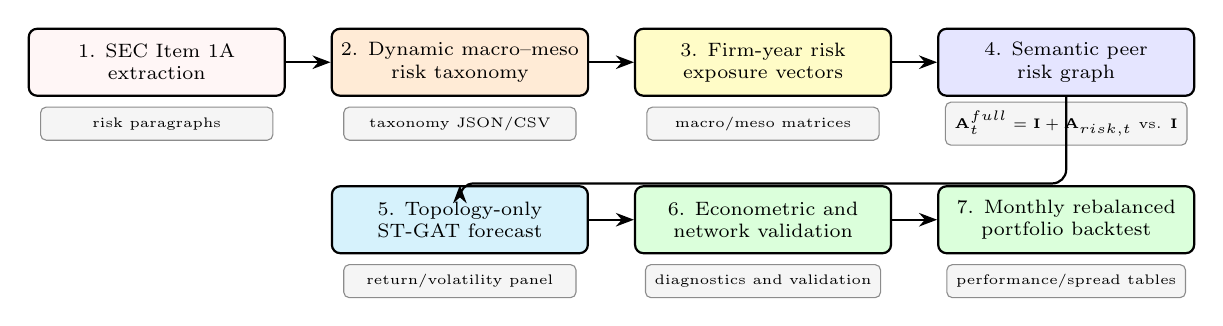
\begin{tikzpicture}[
    stage/.style={rectangle, rounded corners=3pt, draw=black, thick, align=center, minimum width=3.25cm, minimum height=0.85cm, font=\scriptsize},
    note/.style={rectangle, rounded corners=2pt, draw=black!45, align=center, minimum width=2.95cm, minimum height=0.42cm, font=\tiny, fill=gray!8},
    arrow/.style={thick, -{Stealth[length=2.3mm]}},
    softarrow/.style={thick, rounded corners=5pt, -{Stealth[length=2.3mm]}}
]
    \node[stage, fill=pink!14] (sec) at (0,0) {1. SEC Item 1A\\extraction};
    \node[stage, fill=orange!16] (tax) at (3.85,0) {2. Dynamic macro--meso\\risk taxonomy};
    \node[stage, fill=yellow!22] (score) at (7.7,0) {3. Firm-year risk\\exposure vectors};
    \node[stage, fill=blue!10] (graph) at (11.55,0) {4. Semantic peer\\risk graph};

    \node[stage, fill=cyan!16] (gat) at (3.85,-2.0) {5. Topology-only\\ST-GAT forecast};
    \node[stage, fill=green!14] (econ) at (7.7,-2.0) {6. Econometric and\\network validation};
    \node[stage, fill=green!14] (port) at (11.55,-2.0) {7. Monthly rebalanced\\portfolio backtest};

    \node[note] at (0,-0.78) {risk paragraphs};
    \node[note] at (3.85,-0.78) {taxonomy JSON/CSV};
    \node[note] at (7.7,-0.78) {macro/meso matrices};
    \node[note] at (11.55,-0.78) {$\mathbf{A}^{full}_t=\mathbf{I}+\mathbf{A}_{risk,t}$ vs. $\mathbf{I}$};
    \node[note] at (3.85,-2.78) {return/volatility panel};
    \node[note] at (7.7,-2.78) {diagnostics and validation};
    \node[note] at (11.55,-2.78) {performance/spread tables};

    \draw[arrow] (sec) -- (tax);
    \draw[arrow] (tax) -- (score);
    \draw[arrow] (score) -- (graph);
    \draw[softarrow] (graph.south) -- ++(0,-1.1) -| (gat.north);
    \draw[arrow] (gat) -- (econ);
    \draw[arrow] (econ) -- (port);
\end{tikzpicture}
}
\caption[End-to-end research pipeline]{Conceptual end-to-end research pipeline. The diagram is schematic; empirical outputs are generated by the scripts and CSV artifacts listed in the repository output manifest.}
\label{fig:end_to_end_pipeline}
\end{figure}

\subsection{Contributions}
\begin{itemize}
    \item \textbf{LLM-driven hierarchical taxonomy with dynamic evolution:} The project implements a macro--meso taxonomy update mechanism that can add new categories, merge emerging clusters into existing nodes, and reorganize parent macro assignments. Coverage-percentage diagnostics are treated as a reproducibility extension unless their source calculation is regenerated.
    \item \textbf{Topology-only ST-GAT with strict spatial ablation:} The main forecasting model uses $\mathbf{A}_{t}=\mathbf{I}+\mathbf{A}_{risk,t}$, where off-diagonal edges are selected by thresholded cosine similarity of risk exposure vectors. The identity baseline uses $\mathbf{A}_{t}=\mathbf{I}$, isolating the incremental contribution of textual peer topology.
    \item \textbf{Macro-versus-Meso semantic resolution comparison:} Meso-level risk topology produces sparse, high-confidence semantic peer links and outperforms the identity baseline across return and volatility metrics. Macro topology is substantially denser and produces mixed results, improving return ranking but not volatility ranking.
    \item \textbf{Dynamic portfolio extension:} Annual ST-GAT forecasts are converted into monthly rebalanced long-only and long-short portfolios. The best Meso ST-GAT return-only long-short portfolio achieves a Sharpe ratio of 1.06, maximum drawdown of -6.90\%, and a nominally significant annualized top-minus-bottom spread of 17.69\% before multiple-testing adjustment.
    \item \textbf{Multi-model validation:} Integration of LLM taxonomy construction, ST-GAT forecasting, portfolio backtesting, and supplemental EGARCH-X/DAV, Fama-MacBeth, and network diagnostic modules. Source-table-limited econometric outputs are reported as methodology extensions rather than headline evidence.
\end{itemize}

\subsection{Report Organization}
The remainder of this report is organized as follows. Section 2 reviews financial textual analysis, SEC risk disclosure studies, graph neural networks, volatility modeling, and cross-sectional asset-pricing validation. Section 3 describes the data sources and preprocessing pipeline, including risk-factor extraction and the enhanced macro-financial feature matrix. Section 4 details the base-year taxonomy construction and LLM-driven dynamic taxonomy update mechanism. Section 5 formally defines the ST-GAT architecture, including graph construction, identity-matrix ablation, spatial attention, temporal convolution, and masked multi-task loss. Section 6 specifies the tensor construction, train-only standardization, active-mask logic, and feature-target alignment. Section 7 presents the chronological experimental design, Optuna tuning process, and hyperparameter configurations. Section 8 reports forecasting results and graph-density diagnostics. Section 9 introduces the dynamic portfolio backtesting extension, including monthly rebalancing, transaction costs, score ablations, and top-minus-bottom spread diagnostics. Sections 10 and 11 discuss limitations and conclude. Supplemental econometric baseline evaluations (DAV, Fama-MacBeth, and SAR models) and a representative sample of the evolved taxonomy are provided in the Appendices.

% ==========================================
% 2: LITERATURE REVIEW
% ==========================================
\section{LITERATURE REVIEW}

\subsection{Textual Analysis in Finance: From Dictionaries to LLMs}
Lexicon-based methods measure sentiment using pre-defined word lists but cannot capture context, negation, or industry-specific meanings \citep{loughran2011liability, li2010textual}. Topic modeling methods such as Latent Dirichlet Allocation discover latent themes but require a pre-specified number of topics and ignore hierarchical structure \citep{blei2003latent, bao2014simultaneously}. Transformer-based LLMs overcome many of these limitations by learning bidirectional contextual representations \citep{devlin2019bert, liu2019roberta, beltagy2020longformer}. Recent financial-text benchmarks and working papers further motivate domain-specific LLM evaluation on SEC filings \citep{choi2026llm, jiang2026finrate}.

\noindent\textbf{Gap 2.1:} No prior work systematically compares multiple LLM architectures (DeepSeek-R1, GPT-4o-Mini, Llama-3.1) for hierarchical risk taxonomy classification of Item 1A, nor evaluates multi-level prompting strategies.

\subsection{Empirical Studies of SEC Item 1A Risk Factor Disclosures}
Prior accounting and finance studies establish that SEC Item 1A risk-factor disclosures contain market-relevant information. \citet{kravet2013textual} find that changes in risk disclosures are associated with investors' risk perceptions, while \citet{hope2016benefits} show that more specific risk disclosures trigger stronger market responses. \citet{campbell2014information} document the information content of mandatory risk-factor disclosures, and \citet{dyer2017evolution} document the rising length, boilerplate, and stickiness of 10-K text over time. \citet{grundy2021risk} apply sentence-level LDA to S\&P 1500 firms and show that quantified risk-factor text explains a meaningful fraction of cross-sectional risk variation. However, no prior study has systematically quantified year-over-year cosine drift in risk vectors or linked zero-drift boilerplate firms to the performance of graph-based predictive models.

\noindent\textbf{Gap 2.2:} The phenomenon of exactly zero drift (e.g., GE, NTAP) and its role in GNN underperformance has not been empirically established.

\subsection{Graph Neural Networks (GNNs) in Financial Forecasting}
Graph neural networks propagate information over non-Euclidean structures and have become a natural tool for modeling relational dependence \citep{velickovic2018graph}. Spatio-temporal graph attention architectures have also been applied to financial volatility forecasting and risk modeling by propagating information through graphs of interconnected assets \citep{kumar2024temporal}. Existing financial GNN studies typically construct graphs from industry classifications, historical correlations, supply-chain relations, or other static proxies. \citet{niu2024dynamic} emphasize that static graph construction can fail to capture the evolving nature of financial relationships.

\noindent\textbf{Gap 2.3:} No prior study has constructed a graph directly from the semantic content of 10-K risk disclosures, systematically compared macro- versus meso-level graph resolutions, or performed a strict ablation study (replacing the graph with an identity matrix) to isolate the contribution of network topology.

\subsection{Volatility Modeling with Textual Features}
GARCH and EGARCH models capture volatility clustering and leverage effects in asset returns \citep{bollerslev1986generalized, nelson1991conditional}. Extensions such as GARCH-X and EGARCH-X allow exogenous variables to enter the conditional variance equation \citep{naimoli2023realized}. A few studies have incorporated news-based sentiment or information volume, but the frequency mismatch between annual risk disclosures and daily volatility has received little attention.

\noindent\textbf{Gap 2.4:} No prior work systematically documents how annual risk scores, when repeated daily, are absorbed into the long-run variance intercept, nor provides a diagnostic framework (BIC, Diebold-Mariano, Mincer-Zarnowitz) to identify when textual features add value versus add noise.

\subsection{Cross-Sectional Asset Pricing with Textual Features}
The Fama-MacBeth two-step procedure is the standard methodology for testing whether a firm characteristic commands a cross-sectional risk premium \citep{fama1973risk}. \citet{gao2016text} proposes a text-implied risk factor using language-model embeddings, and later disclosure-risk factor studies extend traditional factor models with textual risk signals \citep{stevens2020financial}. \citet{lopezlira2019risk} also shows that textual risk factors can be informative for the cross-section of returns. However, these approaches have not been applied to LLM-derived hierarchical risk scores from Item 1A.

\noindent\textbf{Gap 2.5:} The Fama-MacBeth framework has never been used to test whether LLM-based risk scores from 10-K filings explain cross-sectional variation in returns after controlling for size, momentum, and trailing volatility.

\subsection{Research Gap and the Present Contribution}
Synthesizing the existing literature, four interconnected gaps remain: (i) the absence of quantitative metrics for year-over-year textual drift linked to predictive performance; (ii) the lack of semantic-similarity graph architectures with rigorous spatial ablation protocols; (iii) the absence of a diagnostic framework to address the frequency mismatch between annual disclosures and daily volatility; and (iv) a lack of Fama-MacBeth validation for LLM-derived risk scores from SEC Item 1A.

The present research addresses these gaps by integrating an LLM-driven dynamic taxonomy, a multi-resolution topology-only ST-GAT architecture, and a suite of supplemental validation models. The main forecasting result is that the granular Meso-level topology outperforms the identity baseline across both return and volatility targets in the exported 2021--2024 review-submission OOS panel. The Meso ST-GAT improves averaged RMSE from 0.3345 to 0.3001 and averaged Spearman rank correlation from -0.0139 to 0.1701. For volatility specifically, the Meso ST-GAT reduces RMSE from 0.2240 to 0.1565 and improves Spearman rank from -0.1351 to 0.1770. The portfolio extension is economically suggestive in an academic backtest: the Meso ST-GAT return-only long-short strategy achieves a Sharpe ratio of 1.06 and a nominally significant annualized top-minus-bottom spread of 17.69\% ($p=0.034$) before multiple-testing adjustment. Supplemental DAV peak diagnostics are retained as event-local evidence, while DAV BIC, Fama-MacBeth, and SAR modules are framed as deferred validation extensions when source tables are absent. The central verified contribution is the strict identity-matrix ablation showing that granular textual-risk topology adds predictive information beyond own-firm features alone.
% ==========================================
% 3: DATA & PRE-PROCESSING
% ==========================================
\section{DATA \& PRE-PROCESSING}

\subsection{Data Sources}
Our data pipeline draws from four primary sources:
\begin{itemize}
    \item \textbf{SEC EDGAR Database:} The primary source of textual risk disclosures is the SEC's Electronic Data Gathering, Analysis, and Retrieval (EDGAR) system. We access filings through the SEC's RESTful API, which provides structured access to company filing histories.
    \item \textbf{Yahoo Finance / yfinance:} Daily adjusted prices, volumes, market proxies, and benchmark prices are used in the implemented forecasting feature-generation and portfolio-backtesting modules, including the SPY benchmark equity curve.
    \item \textbf{Market and macro proxies:} The implemented feature matrix includes S\&P 500 return/volatility, VIX level/change, and a 10-year Treasury yield proxy over the same July-to-June feature window.
    \item \textbf{Supplemental data references:} Some appendix experiments reference Fama-MacBeth, DAV/EGARCH-X, and network diagnostics. Where the repository does not contain a parseable source table, the report treats the associated outputs as deferred validation items rather than confirmed findings.
\end{itemize}

\subsection{Sample Description}
All models in this study are trained and validated on the same unified dataset to ensure comparability across approaches. We construct a single, comprehensive sample that serves all modeling tasks.

\textbf{Sample Construction.} The current repository artifacts cover the 2006--2024 risk-year panel. The macro and meso risk-score matrices contain 2,387 firm-year rows across 485 unique tickers, and the enhanced financial feature/target matrix contains 2,367 firm-year rows across 482 unique tickers after target-availability filtering. These counts are taken from the current CSV artifacts under \codepath{data/interim/scoring_outputs}. This sample size is sufficient for:
\begin{itemize}
    \item Training the ST-GAT model with adequate historical sequence data.
    \item Performing validation across diverse firm types and time periods.
    \item Constructing meaningful risk networks with sufficient node connectivity.
\end{itemize}

\textbf{Sample Attributes.}
\begin{itemize}
    \item Time Period: 2006-2024 (18 years)
    \item Number of Firms: 485 tickers in the risk-score matrices; 482 tickers in the enhanced financial matrix
    \item Risk-score Firm-Year Observations: 2,387
    \item Financial feature/target Firm-Year Observations: 2,367
    \item Paragraph-level corpus: stored in the interim master risk-factor file; the final report does not make a standalone paragraph-count claim because the validation suite focuses on firm-year exposure matrices.
\end{itemize}

\textbf{Data Quality Assurance.} To ensure data quality:
\begin{itemize}
    \item Pre-2018 filings with non-standard HTML are bypassed due to parsing inconsistencies.
    \item Survivorship bias is partially mitigated where historical constituents and delisted tickers are available; a fully survivorship-bias-free reconstruction remains a limitation of the academic data environment.
    \item Duplicate filings (amendments, corrected versions) are identified by accession number and deduplicated, retaining only the most recent version.
    \item Irrecoverable filings are excluded from the sample and documented.
\end{itemize}

\textbf{Market Timing Convention.} The implemented ST-GAT task is annual rather than event-day based. For risk year $t$, annual risk exposures and financial features are aligned to the July-to-June feature window, and forward targets are measured over the following July-to-June window. Filing-date event timing is not used in the current ST-GAT output files and should not be interpreted as part of the validated forecasting design.

\subsection{Data Pipeline: Four-Stage Extraction Process}
The data pipeline consists of four sequential stages, each designed to progressively refine raw SEC filings into structured, analyzable risk disclosures.

\textbf{Stage 1: Data Acquisition (Downloading HTML)} \\
\textbf{Objective:} Download the complete annual reports (10-K forms) for a target list of major companies. \\
\textbf{Source:} SEC's EDGAR database at data.sec.gov. \\
\textbf{Input:} A curated list of company tickers (e.g., AAPL, MSFT, TSLA) and their corresponding CIK numbers (unique identifiers used by the SEC). \\
\textbf{Process:} The script sends an HTTP request to the SEC API for each company's submissions history; finds the most recent filing where the form type is 10-K; extracts the URL for the primary HTML document; downloads the entire HTML content. \\
\textbf{Output:} Raw HTML files saved locally (e.g., AAPL\_10K.html).\\

\textbf{Stage 2: Data Extraction (Isolating ``Item 1A'')} \\
\textbf{Objective:} Extract only the ``Item 1A: Risk Factors'' section from the large 10-K HTML files. \\
\textbf{Why this is needed:} A 10-K filing is very large; we need to discard irrelevant sections. \\
\textbf{Process:} Read HTML using an HTML parser; find boundaries with patterns like ``Item 1A Risk Factors''; remove Table of Contents references; locate end point (next item, usually ``Item 1B''); extract HTML elements between boundaries. \\
\textbf{Output:} New HTML files containing only the Risk Factors section. \\

\textbf{Stage 3: Data Structuring (Separating Headings from Descriptions)} \\
\textbf{Step 3.1: Structural Formatting Analysis.} Parse the HTML structure; identify bold text, italic/underlined text, and regular text. Group consecutive bold text as potential Risk Title, following regular text as Risk Description. \\
\textbf{Step 3.2: Frequency-Based Validation (Format Frequency Heuristic).} Filter false positives (section numbers, introductory phrases, legal qualifiers, boilerplate) by analyzing frequency of each formatting type across the document. Core principle: frequency inversely indicates hierarchical level---bolded text appears least frequently (main headings), bold-italic or underlined appears moderately (subheadings), regular text appears most frequently (descriptions). Implementation: count formatting types; classify lowest frequency as main headings, medium as subheadings, highest as descriptions; filter identical repeated phrases; cross-validate with position. \\

\textbf{Stage 4: Data Export (Creating CSV Files)} \\
Iterate files, parse and clean text, flatten hierarchical data into a table, aggregate into a master CSV. Output includes individual CSV files per company, a master CSV with all risks, and summary reports. Final columns: Filename, Company Ticker, Year, Risk Heading, Paragraph Text. \\

\subsection{Macro-Financial Feature Space}
The final ST-GAT feature matrix contains $F=12$ node-level inputs. Firm-level features are computed over the July-to-June feature window associated with each risk year, while market-wide overlays are computed over the same window and shared across firms in that year.

\textbf{Idiosyncratic Metrics (Firm-Specific):}
\begin{itemize}
    \item Annualized realized volatility over the feature window (Vol).
    \item Annualized downside volatility computed from negative daily log returns (\texttt{Downside\_Vol}).
    \item Price deviation from the trailing 200-day moving average (\texttt{MA\_200\_Ratio}).
    \item Eleven-month momentum, excluding the most recent month (\texttt{Momentum\_11M}).
    \item Average dollar trading volume (\texttt{Dollar\_Volume}).
    \item Log-transformed dollar trading volume (\texttt{Log\_Dollar\_Volume}).
\end{itemize}

\textbf{Market and Macro Proxies:}
\begin{itemize}
    \item S\&P 500 cumulative return and realized volatility: \texttt{SP500\_Ret} and \texttt{SP500\_Vol}.
    \item Average VIX level and VIX change over the feature window: \texttt{VIX\_Avg} and \texttt{VIX\_Change}.
    \item Average 10-year Treasury yield proxy and yield change: \texttt{TenY\_Yield\_Avg} and \texttt{TenY\_Yield\_Change}.
\end{itemize}

\textbf{Forward Targets.} The target variables are one-period-ahead cumulative return and annualized volatility over the following July-to-June window. Thus, for risk year $t$, input features and risk topology are observed over July $t$ to June $t+1$, while $\text{Target\_Ret}$ and $\text{Target\_Vol}$ are measured over July $t+1$ to June $t+2$.

\textbf{Feature Standardization.} To prevent look-ahead bias, all node features are standardized using the training split only. Means, standard deviations, and median-imputation values are fitted on 2006--2016 data and then applied unchanged to validation and test regimes.

\section{CONSTRUCTION OF BASE YEAR TAXONOMY AND DYNAMIC UPDATE TAXONOMY}

\subsection{Conceptual Framework of the Dynamic Taxonomy}

The core innovation of this research lies in the transition from static, industry-defined risk classifications to a Dynamic Taxonomy. Traditional classification models frequently suffer from ``semantic decay,'' a phenomenon where emergent risks—such as the rapid rise of generative Artificial Intelligence (AI) or evolving Environmental, Social and Governance (ESG) mandates—are misclassified into broad, outdated categories that fail to capture their specific implications. Furthermore, traditional systems often require intensive manual intervention from financial experts to define and update default risk categories, a process that is both time-consuming and prone to subjective bias.

To address this, we propose a dynamic taxonomy with two components: (i) a base taxonomy constructed from a reference year (2006) using unsupervised hierarchical clustering, and (ii) an evolutionary update mechanism that processes new annual data to add, merge, or reorganize categories when semantic deviation exceeds a threshold ($\theta = 0.45$ cosine similarity). This framework ensures the taxonomy remains data-driven without manual intervention.

\subsection{Base Year Taxonomy Construction}

The base taxonomy is built via a multi-stage pipeline, as detailed below.

\subsubsection{Contextual Encoding}

Each risk factor is represented by concatenating its Headings, Subheadings, and Raw Text fields into a full\_context string. This preserves the structural hierarchy of the 10-K disclosure. We then generate 384-dimensional embeddings using the all-MiniLM-L6-v2 sentence transformer, following the sentence-embedding approach introduced by \citet{reimers2019sentencebert}. This model balances computational efficiency with semantic sensitivity.

\subsubsection{Two-Stage Hierarchical Clustering}
\textbf{Macro-level clustering:}
\begin{itemize}
\item Dimensionality Reduction: UMAP with n\_neighbors=15, min\_dist=0.1, and n\_components=5 is utilized to compress the 384-dimension embeddings into a lower-dimensional manifold (5 components). UMAP is designed to preserve local manifold structure, which is essential for effective density detection \citep{mcinnes2018umap}.
\item Density-based clustering: HDBSCAN with min\_cluster\_size=10 and min\_samples=5 is applied to identify clusters of varying densities and shapes \citep{campello2013density}.
\item This yields macro risk categories (e.g., ``Supply Chain Risk'', ``Regulatory Compliance'').
\end{itemize}
\textbf{Meso-level clustering (within each macro cluster):}
\begin{itemize}
\item For each macro cluster, we extract its embeddings and apply UMAP again (n\_neighbors=8, min\_dist=0.2, n\_components=8).

\item HDBSCAN with min\_cluster\_size=5 and min\_samples=3 identifies meso subcategories.

\item Meso categories are specific risk themes (e.g., ``Cross-Border Data Transfer'', ``Technology Standardization'').
\end{itemize}

\subsubsection{Refined Hybrid Centroids}

For each discovered category (macro or meso), we compute a hybrid centroid that combines data-driven and semantic signals:

\begin{equation}
\mathbf{C}_{\text{refined}} = 0.7 \times \mathbf{X}_{\text{mean}} + 0.3 \times \mathbf{X}_{\text{LLM}}
\end{equation}

where:
\begin{itemize}
\item $\mathbf{X}_{\text{mean}}$ represents the arithmetic mean of all embeddings assigned to the category.
\item $\mathbf{X}_{\text{LLM}}$ represents the embedding of a Centroid Summary generated by an LLM (DeepSeek) from a sample of category members. The prompt asks the LLM to produce a 50-word synthesis of the category's core ``DNA''.
\end{itemize}
The weights (0.7 / 0.3) are heuristic; they prioritize empirical data while anchoring the centroid to human-interpretable semantics, preventing drift caused by outliers.

\subsubsection{Handling Unclassified (“Noise”) Points}

After meso clustering, any risk factor not assigned to a meso category is force-assigned to the nearest meso centroid using cosine similarity. This ensures 100\% coverage for downstream risk exposure vector construction.

\subsection{Dynamic Taxonomy Update (Year-over-Year)}

The evolutionary pipeline processes new-year data (e.g., 2007) and updates the taxonomy from the previous year (e.g., 2006). The workflow consists of four steps.

\subsubsection{Initial Classification and Deviation Detection}

Each new risk factor is embedded and compared to all existing meso centroids from the base taxonomy. The highest cosine similarity is recorded. If that similarity falls below a predefined threshold $\theta = 0.45$, the factor is flagged as a semantic deviation. The threshold was chosen empirically based on the 5th percentile of intra-category similarities in the training set.

\subsubsection{Clustering Deviations}

All deviation points are collected. If the number of deviations is at least the configured minimum meso cluster size of five, they are projected via UMAP and clustered with HDBSCAN. Each resulting cluster represents a candidate new risk theme.

\subsubsection{LLM-Driven Evolution Decision}

For each deviation cluster, we provide the LLM with:
\begin{itemize}
\item Sample texts from the cluster,
\item The top-3 closest existing categories (by cosine similarity),
\item A summary of the current taxonomy.
\end{itemize}
The LLM chooses one of three actions (coded as A, B, C in the prompt):

\begin{table}[h]
\centering
\caption{Decision types for taxonomy evolution}
\begin{tabular}{@{}clp{8cm}@{}}
\toprule
\textbf{Decision} & \textbf{Action} & \textbf{Description} \\
\midrule
A & ADD & Create a new meso category. The LLM provides a recommended name and parent macro category. \\
B & MERGE & Absorb the deviation cluster into the closest existing category. The existing centroid is updated via an exponential moving average (80\% old, 20\% new) to reflect drift. \\
C & REORGANIZE & Move an existing meso category to a different macro parent. The LLM specifies the target category name and the new parent macro. \\
\bottomrule
\end{tabular}
\end{table}

\subsubsection{Execution and Persistence}
\begin{itemize}
\item \textbf{ADD:} A new meso category is appended to the taxonomy with a refined hybrid centroid ($0.7 \times$ math centroid of the cluster $+ 0.3 \times$ embedding of the LLM-recommended name). All deviation points in that cluster are labeled with the new category.

\item \textbf{MERGE:} The closest existing category's centroid is updated to $0.8 \times$ old\_centroid $+ 0.2 \times$ cluster\_math\_centroid, preserving stability while adapting to new data.

\item \textbf{REORGANIZE:} The parent\_macro field of the target category is updated.
\end{itemize}

\subsection{Validation Design and Deferred Coverage Audit}

To evaluate the effectiveness of the proposed dynamic taxonomy, the intended design compares the base taxonomy (built from 2022 data) against the evolved taxonomy (after processing 2024 data). Two validation approaches are specified: (i) a quantitative coverage analysis measuring the reduction of ambiguous classifications, and (ii) a qualitative firm-level case study illustrating how risk profiles shift over time.

\textbf{Repository verification note.} The repository contains the taxonomy JSON/CSV and a coverage-improvement figure, but it does not contain the standalone source table or script output required to reproduce the percentage labels in that figure. The final review report therefore uses the figure only as a conceptual diagnostic of the intended audit and does not treat the specific percentages as headline evidence.

\subsubsection{Coverage Improvement: Baseline vs. Evolved Taxonomy}

For each risk factor in a given year, the intended coverage audit computes cosine similarity to the closest meso-category centroid. A factor is flagged as ``ambiguous/outlier'' if its maximum similarity falls below the deviation threshold $\theta = 0.45$ (as defined in Section 4.3.1). The percentage of factors with similarity $\ge 0.45$ would then provide a direct measure of taxonomic coverage. Because the source table behind the current coverage figure is absent from the reproducibility manifest, this report does not claim a verified coverage improvement value. A full reproducible taxonomy-coverage audit is left as a final validation extension.

\begin{figure}[htbp]
    \centering
    \includegraphics[width=0.5\textwidth]{taxonomy_coverage_improvement.png}
    \caption{Taxonomy coverage improvement--baseline (2022) vs. evolved (2024). This existing figure is retained as a conceptual diagnostic of the intended audit; the final report does not use its percentage labels as headline evidence without the standalone source table.}
    \label{fig:example}
\end{figure}

\subsubsection{Firm-Level Risk Profile Evolution: Case Study}

Beyond aggregate metrics, the dynamic taxonomy enables tracking of individual firms' risk exposure vectors over time. For each year, a firm-level risk exposure vector can be constructed by normalizing the count of risk factors assigned to each meso category by the firm's total number of risk factors. The earlier AAPL migration example is not treated as an empirical result in this final report because the regenerated radar chart and source table are absent from the reproducibility manifest. It is retained only as a description of a feasible case-study design: once regenerated, the analysis should compare AAPL's 2022 and 2024 meso exposure vectors directly and report the exact categories, weights, and source rows.

\subsubsection{Discussion of Validation}

Subject to regeneration of the coverage source table and firm-level case-study plot, the taxonomy validation extension would test whether:
\begin{itemize}
\item a fixed taxonomy loses coverage over a multi-year horizon;
\item the evolutionary mechanism mitigates semantic decay by detecting deviation clusters and applying ADD/MERGE/REORGANIZE decisions; and
\item evolved risk exposure vectors become more specialized in ways that reflect actual changes in disclosure content.
\end{itemize}
Limitations: The validation is limited to two time points (2022 and 2024). A full longitudinal study (e.g., rolling updates from 2015 to 2024) would be required to assess long-term stability. Additionally, the coverage metric relies on the fixed similarity threshold (0.45); sensitivity analysis on this threshold is left for future work.

% ==========================================
\section{MATHEMATICAL FORMULATION OF THE SPATIO-TEMPORAL ARCHITECTURE}
% ==========================================
The predictive objective of the ST-GAT model is to determine whether semantic similarity in annual SEC Item 1A risk disclosures provides cross-sectional information beyond each firm's own financial trajectory. The architecture is therefore designed as a strict spatial ablation. The full model uses a dynamic risk-similarity topology, while the baseline uses only self-loops. This section defines the graph, attention mechanism, temporal convolution layer, masking logic, and multi-task loss used for one-year-ahead return and volatility prediction.

% --- CLEAN ST-GAT BLOCK ARCHITECTURE FIGURE ---
\begin{figure}[H]
\centering
\resizebox{0.96\textwidth}{!}{
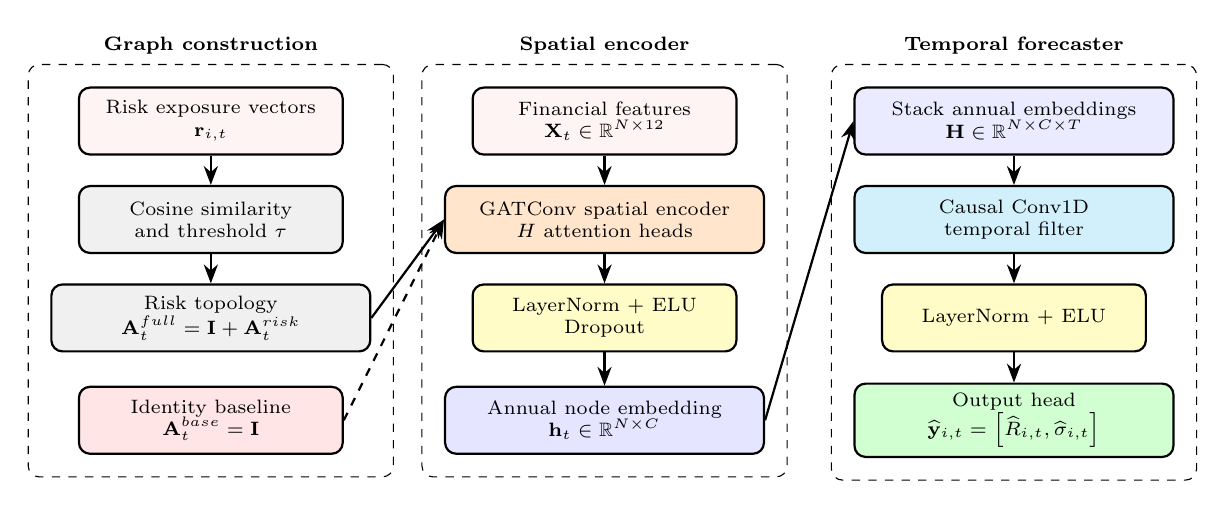
\begin{tikzpicture}[
    block/.style={rectangle, rounded corners, draw=black, thick, align=center, minimum width=3.35cm, minimum height=0.85cm, font=\scriptsize},
    wideblock/.style={rectangle, rounded corners, draw=black, thick, align=center, minimum width=4.05cm, minimum height=0.85cm, font=\scriptsize},
    group/.style={rectangle, rounded corners, draw=black, dashed, inner sep=0.28cm},
    arrow/.style={thick, -{Stealth[length=2.4mm]}},
    dashedarrow/.style={thick, dashed, -{Stealth[length=2.4mm]}}
]
    % Column 1: graph construction
    \node[block, fill=pink!18] (risk) at (0,0) {Risk exposure vectors\\$\mathbf{r}_{i,t}$};
    \node[block, fill=gray!12] (cosine) at (0,-1.25) {Cosine similarity\\and threshold $\tau$};
    \node[wideblock, fill=gray!12] (adj) at (0,-2.50) {Risk topology\\$\mathbf{A}^{full}_{t}=\mathbf{I}+\mathbf{A}^{risk}_{t}$};
    \node[block, fill=red!10] (base) at (0,-3.80) {Identity baseline\\$\mathbf{A}^{base}_{t}=\mathbf{I}$};

    % Column 2: spatial encoder
    \node[block, fill=pink!18] (features) at (5.0,0) {Financial features\\$\mathbf{X}_{t}\in\mathbb{R}^{N\times 12}$};
    \node[wideblock, fill=orange!20] (gat) at (5.0,-1.25) {GATConv spatial encoder\\$H$ attention heads};
    \node[block, fill=yellow!22] (norm) at (5.0,-2.50) {LayerNorm + ELU\\Dropout};
    \node[wideblock, fill=blue!10] (emb) at (5.0,-3.80) {Annual node embedding\\$\mathbf{h}_{t}\in\mathbb{R}^{N\times C}$};

    % Column 3: temporal forecasting
    \node[wideblock, fill=blue!8] (stack) at (10.2,0) {Stack annual embeddings\\$\mathbf{H}\in\mathbb{R}^{N\times C\times T}$};
    \node[wideblock, fill=cyan!18] (conv) at (10.2,-1.25) {Causal Conv1D\\temporal filter};
    \node[block, fill=yellow!22] (norm2) at (10.2,-2.50) {LayerNorm + ELU};
    \node[wideblock, fill=green!18] (out) at (10.2,-3.80) {Output head\\$\widehat{\mathbf{y}}_{i,t}=\left[\widehat{R}_{i,t},\widehat{\sigma}_{i,t}\right]$};

    % Main arrows
    \draw[arrow] (risk) -- (cosine);
    \draw[arrow] (cosine) -- (adj);
    \draw[arrow] (features) -- (gat);
    \draw[arrow] (gat) -- (norm);
    \draw[arrow] (norm) -- (emb);
    \draw[arrow] (emb.east) -- (stack.west);
    \draw[arrow] (stack) -- (conv);
    \draw[arrow] (conv) -- (norm2);
    \draw[arrow] (norm2) -- (out);

    % Cross-module arrows
    \draw[arrow] (adj.east) -- (gat.west);
    \draw[dashedarrow] (base.east) -- (gat.west);

    % Group labels
    \node[group, fit=(risk)(cosine)(adj)(base), label={[font=\scriptsize\bfseries]above:Graph construction}] {};
    \node[group, fit=(features)(gat)(norm)(emb), label={[font=\scriptsize\bfseries]above:Spatial encoder}] {};
    \node[group, fit=(stack)(conv)(norm2)(out), label={[font=\scriptsize\bfseries]above:Temporal forecaster}] {};

\end{tikzpicture}
}
\caption[ST-GAT architecture and identity ablation]{ST-GAT block architecture and identity-matrix ablation. Risk exposure vectors define the sparse graph topology, financial node features enter the spatial GAT encoder, and annual embeddings are passed through a causal temporal forecaster to predict one-year-ahead return and volatility. The full model uses textual peer topology, whereas the identity baseline removes all off-diagonal links. Cosine similarity determines edge existence, while attention weights are learned by GATConv.}
\label{fig:stgat_architecture}
\end{figure}

% --- TEMPORAL SNAPSHOT TENSOR DIAGRAM ---
\begin{figure}[H]
\centering
\resizebox{0.78\textwidth}{!}{
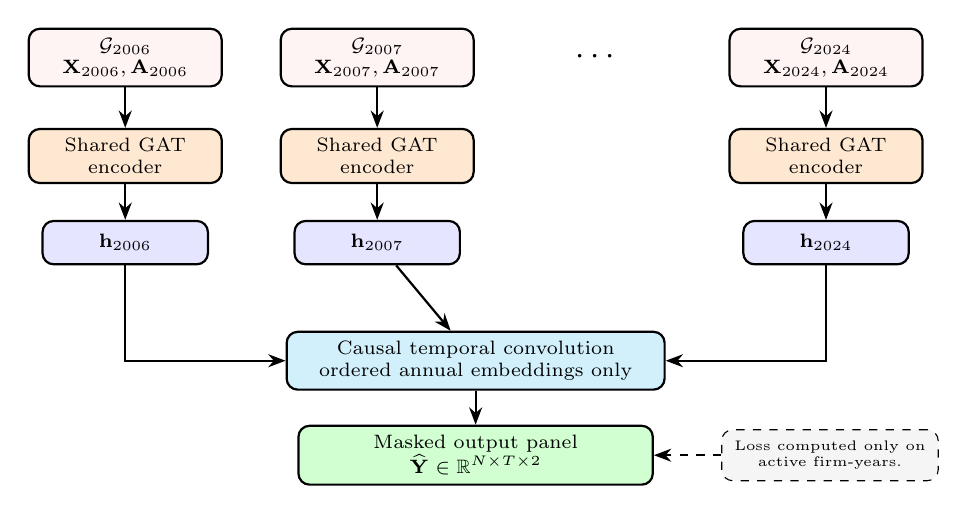
\begin{tikzpicture}[
    snap/.style={rectangle, rounded corners, draw=black, thick, align=center, minimum width=2.45cm, minimum height=0.65cm, font=\scriptsize, fill=pink!18},
    encoder/.style={rectangle, rounded corners, draw=black, thick, align=center, minimum width=2.45cm, minimum height=0.65cm, font=\scriptsize, fill=orange!18},
    embed/.style={rectangle, rounded corners, draw=black, thick, align=center, minimum width=2.10cm, minimum height=0.55cm, font=\scriptsize, fill=blue!10},
    temporal/.style={rectangle, rounded corners, draw=black, thick, align=center, minimum width=4.8cm, minimum height=0.72cm, font=\scriptsize, fill=cyan!18},
    outpanel/.style={rectangle, rounded corners, draw=black, thick, align=center, minimum width=4.5cm, minimum height=0.68cm, font=\scriptsize, fill=green!18},
    ann/.style={rectangle, draw=black, dashed, rounded corners, align=center, font=\tiny, inner sep=4pt, fill=gray!8, minimum width=2.75cm},
    arrow/.style={thick, -{Stealth[length=2.2mm]}},
    dashedarrow/.style={thick, dashed, -{Stealth[length=2.2mm]}}
]
    \node[snap] (x06) at (0,0) {$\mathcal{G}_{2006}$\\$\mathbf{X}_{2006},\mathbf{A}_{2006}$};
    \node[snap] (x07) at (3.2,0) {$\mathcal{G}_{2007}$\\$\mathbf{X}_{2007},\mathbf{A}_{2007}$};
    \node[font=\large] (dots) at (6.0,0) {$\cdots$};
    \node[snap] (x24) at (8.9,0) {$\mathcal{G}_{2024}$\\$\mathbf{X}_{2024},\mathbf{A}_{2024}$};

    \node[encoder] (gat06) at (0,-1.25) {Shared GAT\\encoder};
    \node[encoder] (gat07) at (3.2,-1.25) {Shared GAT\\encoder};
    \node[encoder] (gat24) at (8.9,-1.25) {Shared GAT\\encoder};

    \node[embed] (h06) at (0,-2.35) {$\mathbf{h}_{2006}$};
    \node[embed] (h07) at (3.2,-2.35) {$\mathbf{h}_{2007}$};
    \node[embed] (h24) at (8.9,-2.35) {$\mathbf{h}_{2024}$};

    \node[temporal] (conv) at (4.45,-3.85) {Causal temporal convolution\\ordered annual embeddings only};
    \node[outpanel] (pred) at (4.45,-5.05) {Masked output panel\\$\widehat{\mathbf{Y}}\in\mathbb{R}^{N\times T\times 2}$};
    \node[ann] (mask) at (8.95,-5.05) {Loss computed only on\\active firm-years.};

    \draw[arrow] (x06) -- (gat06);
    \draw[arrow] (x07) -- (gat07);
    \draw[arrow] (x24) -- (gat24);
    \draw[arrow] (gat06) -- (h06);
    \draw[arrow] (gat07) -- (h07);
    \draw[arrow] (gat24) -- (h24);
    \draw[arrow] (h06) |- (conv);
    \draw[arrow] (h07) -- (conv);
    \draw[arrow] (h24) |- (conv);
    \draw[arrow] (conv) -- (pred);
    \draw[dashedarrow] (mask.west) -- (pred.east);
\end{tikzpicture}
}
\caption[Temporal graph snapshot processing]{Temporal processing of annual graph snapshots. The shared GAT encoder is applied to each annual graph, and a causal temporal convolution produces masked return-volatility predictions across the full panel.}
\label{fig:temporal_snapshot_architecture}
\end{figure}

\subsection{Dynamic Risk-Similarity Graph Definition}
For each year $t$, the financial universe is represented as an attributed graph:
\begin{equation}
\mathcal{G}_t = (\mathcal{V}, \mathcal{E}_t, \mathbf{A}_t, \mathbf{X}_t),
\end{equation}
where $\mathcal{V}=\{v_1,\ldots,v_N\}$ is the global node universe, $\mathcal{E}_t$ is the annual edge set, $\mathbf{A}_t \in \mathbb{R}^{N\times N}$ is the adjacency matrix, and $\mathbf{X}_t\in\mathbb{R}^{N\times F}$ is the node feature matrix. In the final implementation, $F=12$ financial and macro-market features are used for each firm-year.

For each firm $i$ and year $t$, the risk exposure vector $\mathbf{r}_{i,t}$ is constructed from normalized paragraph shares:
\begin{equation}
 r_{i,k,t}=\frac{\text{number of Item 1A paragraphs of firm }i\text{ assigned to risk category }k\text{ in year }t}{\text{total Item 1A paragraphs of firm }i\text{ in year }t}.
\end{equation}
Macro graphs use first-level risk categories, while Meso graphs use second-level risk categories. The off-diagonal semantic similarity between firms $i$ and $j$ is computed using cosine similarity:
\begin{equation}
 s_{ij,t}=\frac{\mathbf{r}_{i,t}^{\top}\mathbf{r}_{j,t}}{\|\mathbf{r}_{i,t}\|_2\|\mathbf{r}_{j,t}\|_2}.
\end{equation}
A risk edge is retained only if similarity exceeds an optimizable threshold $\tau$:
\begin{equation}
 A^{risk}_{ij,t}=\begin{cases}
1, & i\neq j \text{ and } s_{ij,t}\geq \tau,\\
0, & \text{otherwise.}
\end{cases}
\end{equation}
The main reported specification is topology-only: cosine similarity determines whether an edge exists, but raw cosine weights are not directly passed into the GAT attention mechanism. This design was selected after weighted-edge attention was found to be less stable empirically. Edge weights are retained for diagnostics and optional ablations, but the primary model allows the GAT layer to learn propagation weights from node features and graph topology.

\subsection{Full Graph versus Identity Baseline}
The final spatial ablation is defined as:
\begin{equation}
\mathbf{A}^{full}_t=\mathbf{I}_N+\mathbf{A}^{risk}_t,
\end{equation}
while the baseline is:
\begin{equation}
\mathbf{A}^{base}_t=\mathbf{I}_N.
\end{equation}
Therefore, the full ST-GAT receives each firm's own information and information from textually similar peers, while the baseline receives only each firm's own information. This establishes a clean test of whether the NLP-derived risk topology contributes predictive information beyond isolated firm-level features.

\begin{table}[H]
\centering
\caption{Adjacency structures used in the ST-GAT ablation.}
\label{tab:adjacency_comparison}
\vspace{0.2cm}
\renewcommand{\arraystretch}{1.35}
\begin{tabular}{p{3.5cm}p{4.5cm}p{6.5cm}}
\toprule
\textbf{Model} & \textbf{Adjacency} & \textbf{Interpretation} \\
\midrule
Full ST-GAT & $\mathbf{A}^{full}_t=\mathbf{I}_N+\mathbf{A}^{risk}_t$ & Own-firm information plus peer spillovers from firms with similar 10-K risk exposure vectors. \\
Identity Baseline & $\mathbf{A}^{base}_t=\mathbf{I}_N$ & Own-firm information only; all off-diagonal textual peer links are removed. \\
\bottomrule
\end{tabular}
\end{table}

\subsection{Spatial Graph Attention Mechanism}
For each annual graph snapshot, a graph attention layer transforms node features into spatial embeddings, following the attention-based neighborhood aggregation principle of Graph Attention Networks \citep{velickovic2018graph}.
\begin{equation}
e_{ij,t}=\text{LeakyReLU}\left(\mathbf{a}^{\top}[\mathbf{W}\mathbf{x}_{i,t}\parallel \mathbf{W}\mathbf{x}_{j,t}]\right),
\end{equation}
where $\mathbf{W}$ is a learnable projection, $\mathbf{a}$ is the attentional vector, and $\parallel$ denotes concatenation. The normalized attention weight is:
\begin{equation}
\alpha_{ij,t}=\frac{\exp(e_{ij,t})}{\sum_{k\in\mathcal{N}_t(i)}\exp(e_{ik,t})}.
\end{equation}
The spatial embedding for node $i$ is then:
\begin{equation}
\mathbf{h}_{i,t}=\sigma\left(\sum_{j\in\mathcal{N}_t(i)}\alpha_{ij,t}\mathbf{W}\mathbf{x}_{j,t}\right).
\end{equation}
Multi-head attention is used to capture distinct modes of peer interaction:
\begin{equation}
\mathbf{h}'_{i,t}=\mathop{\Big\Vert}_{m=1}^{H}\sigma\left(\sum_{j\in\mathcal{N}_t(i)}\alpha^{(m)}_{ij,t}\mathbf{W}^{(m)}\mathbf{x}_{j,t}\right).
\end{equation}
In the implementation, the GAT output is followed by layer normalization, ELU activation, and dropout. Self-loops are supplied explicitly by the data pipeline, so the graph convolution layer is configured without automatic self-loop insertion.

\subsection{Temporal Convolutional Mechanism}
After spatial encoding, annual embeddings are stacked into a temporal tensor:
\begin{equation}
\mathbf{H}\in\mathbb{R}^{N\times C\times T},
\end{equation}
where $C$ is the concatenated spatial embedding dimension and $T$ is the number of annual snapshots. A causal one-dimensional convolution is then applied along the temporal dimension, following the standard temporal-convolution principle that predictions at time $t$ should not depend on future states \citep{bai2018empirical}:
\begin{equation}
\mathbf{z}_{i,t}=\sigma\left(\sum_{k=0}^{K-1}\mathbf{W}_{T}^{(k)}\mathbf{h}'_{i,t-k}+\mathbf{b}_{T}\right).
\end{equation}
The causal truncation ensures that the representation at year $t$ depends only on current and historical graph states. The final output layer maps the temporal representation to two forward targets:
\begin{equation}
\widehat{\mathbf{y}}_{i,t}=\left[\widehat{R}_{i,t},\widehat{\sigma}_{i,t}\right].
\end{equation}

\subsection{Masked Multi-Task Loss}
Because the global universe contains firms that are not active in every year, the model uses a target-aware active mask $M_{t,i}\in\{0,1\}$. A firm-year is active only when it has valid risk exposure data, valid financial features, and non-missing forward return and volatility labels. The training objective is the masked Huber loss averaged over active firm-years. Huber loss is used because it is less sensitive to extreme return observations than squared-error loss while remaining differentiable around zero \citep{huber1964robust}:
\begin{equation}
\mathcal{L}=\frac{1}{|\mathcal{T}|}\sum_{t\in\mathcal{T}}\frac{1}{\sum_i M_{t,i}}\sum_{i=1}^{N}M_{t,i}\,\ell_{\delta}\left(\hat{\mathbf{y}}_{i,t},\mathbf{y}_{i,t}\right),
\end{equation}
where $\ell_{\delta}$ is the Huber loss with $\delta=1.0$. The first output dimension $\widehat{R}_{i,t}$ denotes predicted one-year-ahead cumulative return, and the second output dimension $\widehat{\sigma}_{i,t}$ denotes predicted one-year-ahead annualized volatility. Return and volatility are optimized jointly with equal weight, while evaluation reports target-specific RMSE, MAE, and Spearman rank correlation.

% ==========================================
\section{DATA PIPELINE AND MULTI-DIMENSIONAL TENSOR STRUCTURE}
% ==========================================
The ST-GAT pipeline converts annual risk-score matrices and financial features into a sequence of graph snapshots. Each snapshot contains node features, sparse graph edges, optional edge attributes, forward targets, and an active mask. This section describes the tensor construction and the procedures used to avoid look-ahead bias.

\subsection{Node Feature Engineering and Train-Only Standardization}
For each node $v_i$ and year $t$, the feature vector $\mathbf{x}_{i,t}\in\mathbb{R}^{12}$ consists of six firm-level features and six market or macro proxy features. The twelve inputs are Vol, Downside\_Vol, MA\_200\_Ratio, Momentum\_11M, Dollar\_Volume, Log\_Dollar\_Volume, SP500\_Ret, SP500\_Vol, VIX\_Avg, VIX\_Change, TenY\_Yield\_Avg, and TenY\_Yield\_Change.

Feature preprocessing is fitted only on the training split. Training-year medians are used to impute missing active-node features, and training-year means and standard deviations are used for standardization. The same fitted statistics are then applied to validation and OOS test years. This prevents information from 2017 onward from entering the feature scaling process.

\begin{table}[H]
\centering
\caption{Final ST-GAT node feature set ($F=12$).}
\label{tab:feature_engineering}
\vspace{0.2cm}
\renewcommand{\arraystretch}{1.25}
\small
\begin{tabularx}{\textwidth}{@{}L{3.5cm}Y L{2.6cm}@{}}
\toprule
\textbf{Feature Category} & \textbf{Specific Metrics} & \textbf{Frequency} \\
\midrule
Firm-specific price and risk & \texttt{Vol}; \texttt{Downside\_Vol}; \texttt{MA\_200\_Ratio}; \texttt{Momentum\_11M} & Annual window \\
Firm-specific liquidity & \texttt{Dollar\_Volume}; \texttt{Log\_Dollar\_Volume} & Annual window \\
Market regime & \texttt{SP500\_Ret}; \texttt{SP500\_Vol}; \texttt{VIX\_Avg}; \texttt{VIX\_Change} & Annual window \\
Interest-rate proxy & \texttt{TenY\_Yield\_Avg}; \texttt{TenY\_Yield\_Change} & Annual window \\
\bottomrule
\end{tabularx}
\end{table}

\subsection{Feature-Target Alignment}
The data pipeline follows a July-to-June alignment. For risk year $t$, financial and market features are measured from July 1 of year $t$ to June 30 of year $t+1$. Forward targets are measured from July 1 of year $t+1$ to June 30 of year $t+2$. This matches the annual disclosure cycle while ensuring that the prediction target is strictly forward-looking.

The review-submission results use the current exported 2021--2024 OOS panel, including 2024 rows already present in the repository outputs. Because the risk-year 2024 target window extends to 2026-06-30, final archival results can be refreshed after that window closes; this does not change the review-version comparison logic or the chronological split.

\subsection{Graph Snapshot Tensor Structure}
For each year $t$, the graph builder produces:
\begin{align}
\mathbf{X}_t &\in \mathbb{R}^{N\times F},\\
\mathbf{edge\_index}_t &\in \mathbb{N}^{2\times E_t},\\
\mathbf{edge\_attr}_t &\in \mathbb{R}^{E_t},\\
\mathbf{Y}_t &\in \mathbb{R}^{N\times 2},\\
\mathbf{M}_t &\in \{0,1\}^{N}.
\end{align}
The complete supervised panel is then represented as:
\begin{equation}
\mathbf{Y}\in\mathbb{R}^{N\times T\times 2},\qquad \mathbf{M}\in\{0,1\}^{T\times N}.
\end{equation}
Unlike a random mini-batch design, training is performed on the full chronological graph panel with masked losses. This is appropriate because the graph topology and temporal convolution depend on ordered annual snapshots.

\subsection{Reproducibility and Output Verification}
The repository includes a lightweight validation script that checks canonical artifact paths, CSV schemas, required columns, duplicate firm-years, chronological split labels, train-only preprocessing statistics, graph self-loop logic, identity-baseline edges, portfolio timing, transaction-cost conversion, and deterministic random-number generation:

\begin{verbatim}
.venv/bin/python scripts/validate_pipeline.py --as-of 2026-04-27
\end{verbatim}

The current validation result is 45 passed checks, 2 warnings, and 0 failures. The warnings are: (i) four missing feature values in the enhanced financial matrix are imputed downstream using training-year medians, and (ii) the review panel includes 2024 rows whose final archival target window closes on 2026-06-30. Table \ref{tab:verification_map} summarizes the main source artifacts behind the reported results; exact repository paths are listed in \codepath{docs/output_manifest.md}.

\begin{table}[H]
\centering
\caption{Output verification map for major report claims.}
\label{tab:verification_map}
\vspace{0.2cm}
\footnotesize
\renewcommand{\arraystretch}{1.22}
\setlength{\tabcolsep}{3pt}
\begin{tabularx}{\textwidth}{@{}L{2.55cm}Y Y L{2.15cm}@{}}
\toprule
\textbf{Claim Area} & \textbf{Source Output File} & \textbf{Source Script} & \textbf{Status} \\
\midrule
Macro ST-GAT OOS &
Macro OOS goodness-of-fit CSV &
Macro forecast script &
Verified for review panel \\
Meso ST-GAT OOS &
Meso OOS goodness-of-fit CSV &
Meso forecast script &
Verified for review panel \\
Robust OOS comparison &
Robust OOS evaluation CSV &
Robust OOS evaluation script &
Verified for review panel \\
Graph density &
Macro/meso graph diagnostic artifacts &
Graph pipeline and forecasting scripts &
Verified \\
Portfolio summary and spreads &
Portfolio summary and spread CSVs &
Portfolio backtest script &
Verified \\
Portfolio robust inference &
Portfolio robust-inference CSVs &
Portfolio inference script &
Verified for review panel \\
DAV peak diagnostics &
DAV peak summary CSV and audit note &
DAV peak summary script &
Figure-derived; verified \\
Taxonomy coverage &
Taxonomy coverage figure &
Source table absent &
Deferred audit \\
DAV appendix &
BIC/FMB/SAR plots and tables; source CSV incomplete or absent &
Econometric scripts &
Deferred validation \\
\bottomrule
\end{tabularx}
\end{table}

% ==========================================
\section{EXPERIMENTAL DESIGN AND ALGORITHMIC TUNING}
% ==========================================
The empirical design evaluates whether textual risk topology improves one-year-ahead return and volatility prediction under strict chronological splitting. Random cross-sectional splits are avoided because they would leak future macro regimes into model selection.

\subsection{Strict Chronological Data Splitting}
The sample is split into three non-overlapping temporal regimes:
\begin{itemize}
    \item \textbf{Training Set (2006--2016):} Used to fit model weights, feature standardization statistics, and median imputation values.
    \item \textbf{Validation Set (2017--2020):} Used for Optuna hyperparameter selection and early stopping.
    \item \textbf{Out-of-Sample Test Set (2021--2024):} Used only for final evaluation.
\end{itemize}

\subsection{Dual-Level Spatial Ablation Framework}
Three graph settings are evaluated:
\begin{enumerate}
    \item \textbf{Macro-Level Topology:} Edges are constructed from broad first-level risk category exposure vectors.
    \item \textbf{Meso-Level Topology:} Edges are constructed from granular second-level risk category exposure vectors.
    \item \textbf{Identity Baseline:} All off-diagonal risk edges are removed, leaving only self-loops.
\end{enumerate}
This design tests both whether textual peer topology improves forecasting and whether semantic resolution affects the quality of that topology.

\subsection{Algorithmic Tuning and Optimization}
Macro and Meso graphs have different densities and information bandwidths, so they are tuned independently. We use Optuna with a Tree-structured Parzen Estimator sampler and a Median Pruner, following modern automated hyperparameter optimization practice \citep{akiba2019optuna}. Each study runs 50 trials. The objective minimizes validation Huber loss over 2017--2020, with maximum 200 epochs per trial, patience of 25 epochs, gradient clipping at $1.0$, and early pruning of weak trials. The final forecast models are trained with maximum 300 epochs, patience of 40 epochs, and restoration of the best validation checkpoint.

\begin{table}[H]
\centering
\caption{Optuna search space and final hyperparameters.}
\label{tab:hyperparameters}
\vspace{0.2cm}
\renewcommand{\arraystretch}{1.25}
\resizebox{\textwidth}{!}{
\begin{tabular}{llcc}
\toprule
\textbf{Hyperparameter} & \textbf{Search Space} & \textbf{Macro ST-GAT} & \textbf{Meso ST-GAT} \\
\midrule
Similarity Threshold ($\tau$) & Uniform: $[0.75,0.95]$ & $0.8128$ & $0.8292$ \\
Attention Heads ($H$) & Categorical: $\{1,2,4,8\}$ & $1$ & $2$ \\
Spatial Dimension & Categorical: $\{8,16,32\}$ & $16$ & $8$ \\
Dropout Rate ($p$) & Uniform: $[0.10,0.50]$ & $0.3688$ & $0.4979$ \\
Learning Rate ($\eta$) & Log-uniform: $[10^{-4},10^{-2}]$ & $6.69\times10^{-3}$ & $8.08\times10^{-3}$ \\
Weight Decay & Log-uniform: $[10^{-6},10^{-3}]$ & $1.98\times10^{-5}$ & $5.83\times10^{-5}$ \\
Best Validation Huber Loss & -- & $0.0378$ & $0.0347$ \\
\bottomrule
\end{tabular}
}
\end{table}

\begin{figure}[H]
    \centering
    \begin{minipage}{0.48\textwidth}
        \centering
        \includegraphics[width=\linewidth]{GAT_output_macro/optuna_optimization_history_macro.png}
        \caption{Optimization History (Macro Level)}
    \end{minipage}\hfill
    \begin{minipage}{0.48\textwidth}
        \centering
        \includegraphics[width=\linewidth]{GAT_output_meso/optuna_optimization_history_meso.png}
        \caption{Optimization History (Meso Level)}
    \end{minipage}
    \label{fig:optuna_history}
\end{figure}

\begin{figure}[H]
    \centering
    \begin{minipage}{0.48\textwidth}
        \centering
        \includegraphics[width=\linewidth]{GAT_output_macro/optuna_param_importances_macro.png}
        \caption{Hyperparameter Importance (Macro Level)}
    \end{minipage}\hfill
    \begin{minipage}{0.48\textwidth}
        \centering
        \includegraphics[width=\linewidth]{GAT_output_meso/optuna_param_importances_meso.png}
        \caption{Hyperparameter Importance (Meso Level)}
    \end{minipage}
    \label{fig:param_importance}
\end{figure}

% ==========================================
\section{OUT-OF-SAMPLE PERFORMANCE AND EMPIRICAL RESULTS}
% ==========================================
This section reports OOS predictive performance on the currently exported 2021--2024 review panel. Performance is measured by RMSE, MAE, and Spearman rank correlation. Spearman rank is particularly important because the portfolio extension relies on cross-sectional ranking rather than point forecasts alone.

\begin{figure}[H]
    \centering
    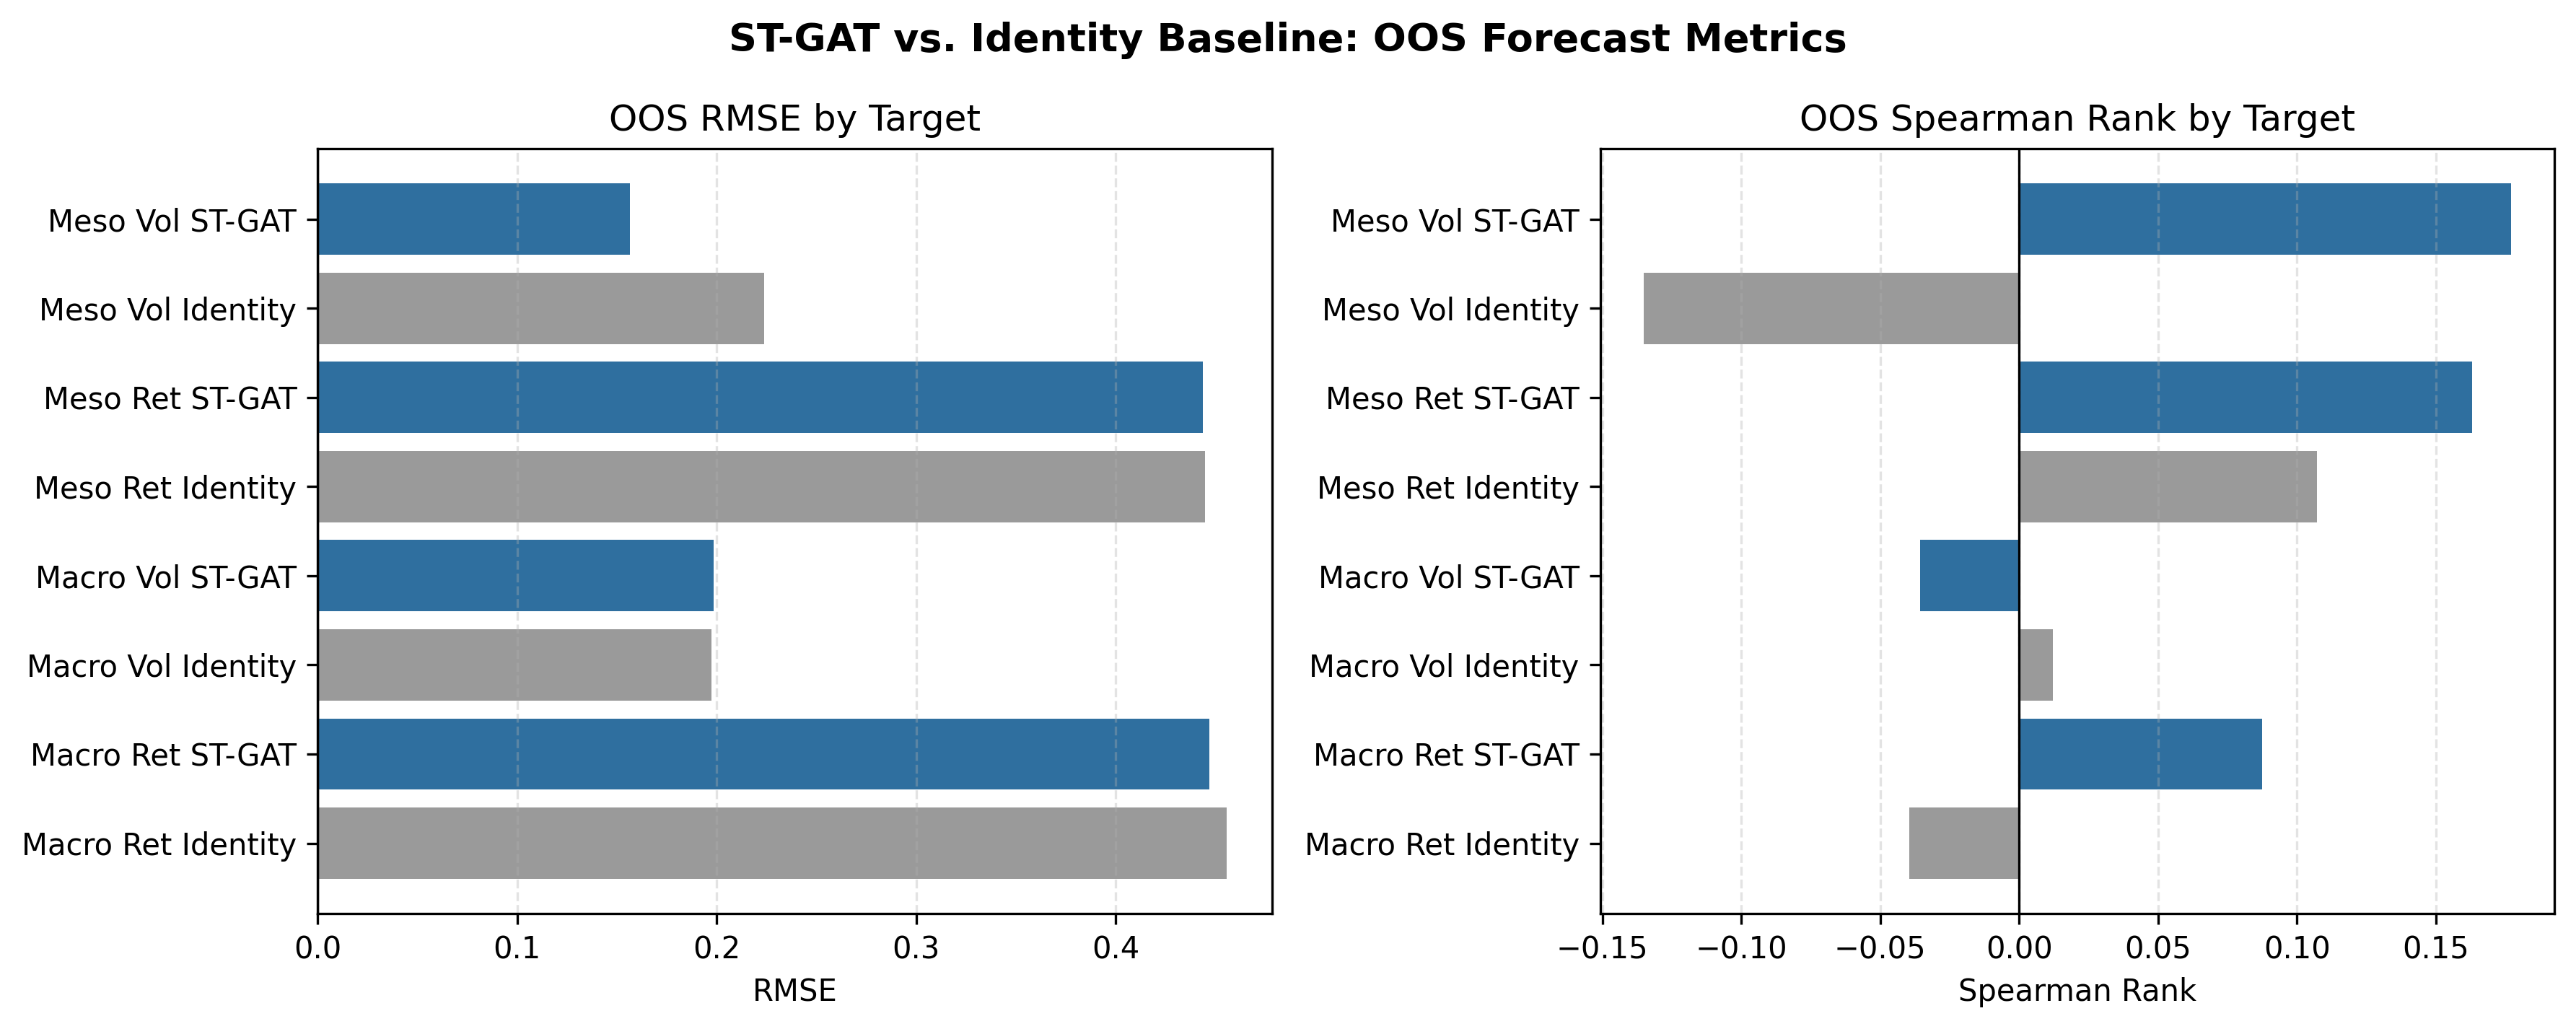
\includegraphics[width=0.98\textwidth]{oos_metric_comparison.png}
    \caption[OOS metric comparison]{Empirical OOS metric comparison generated from \texttt{goodness\_of\_fit\_metrics\_macro\_OOS.csv} and \texttt{goodness\_of\_fit\_metrics\_meso\_OOS.csv}. Lower RMSE is better; higher Spearman rank correlation is better.}
    \label{fig:oos_metric_comparison}
\end{figure}

\subsection{Robust Baseline Comparison}
To avoid over-interpreting point estimates, the repository now includes a robustness addendum generated by \codepath{scripts/evaluate_oos_robustness.py}. The script compares ST-GAT against the identity baseline using paired firm-year errors, year-block bootstrap intervals, and annual-block loss-difference tests. Because the OOS window contains only four risk years, these tests are diagnostic rather than definitive.

\begin{table}[H]
\centering
\caption{Robust OOS improvement diagnostics versus identity baseline. Positive values favor ST-GAT.}
\label{tab:robust_oos}
\vspace{0.2cm}
\renewcommand{\arraystretch}{1.18}
\resizebox{\textwidth}{!}{
\begin{tabular}{llccc}
\toprule
\textbf{Level} & \textbf{Target} & \textbf{RMSE Improvement} & \textbf{MAE Improvement} & \textbf{Spearman Improvement} \\
\midrule
Macro & Return & 0.0087 [$-0.0024$, 0.0151] & 0.0101 [$-0.0134$, 0.0311] & 0.1269 [$-0.1769$, 0.2031] \\
Macro & Volatility & $-0.0011$ [$-0.0555$, 0.0348] & $-0.0026$ [$-0.0572$, 0.0335] & $-0.0477$ [$-0.2456$, 0.1001] \\
Meso & Return & 0.0013 [$-0.0092$, 0.0130] & 0.0059 [$-0.0015$, 0.0138] & 0.0558 [$-0.0361$, 0.1971] \\
Meso & Volatility & \textbf{0.0675 [0.0381, 0.0897]} & \textbf{0.0588 [0.0155, 0.0850]} & \textbf{0.3121 [0.2915, 0.6190]} \\
\bottomrule
\end{tabular}
}
\end{table}

The robust addendum strengthens the main interpretation while narrowing it. The most stable OOS gain is Meso volatility forecasting: all bootstrap confidence intervals are positive, and the annual-block squared-error improvement has a diagnostic $p$-value of 0.040. Return-forecast improvements are directionally positive, especially for rank correlation, but their bootstrap intervals cross zero. Therefore, the strongest statistically defensible claim is not that ST-GAT uniformly dominates the identity baseline across all targets, but that granular Meso topology provides a particularly robust volatility-forecasting advantage and a suggestive return-ranking signal.

\subsection{Seed-Stability Check}
Neural-network results can be sensitive to random initialization. To avoid selecting a favorable seed ex post, the repository includes an optional seed-stability protocol in \codepath{scripts/run_multi_seed_forecasts.py}. The protocol reruns the final forecast stage using the validation-selected Optuna hyperparameters and writes outputs to \codepath{outputs/gat/multi_seed/}, leaving the canonical headline output files unchanged. The current addendum uses seeds 41, 42, and 43.

\begin{table}[H]
\centering
\caption{Final-forecast seed stability across seeds 41, 42, and 43. Values are mean $\pm$ standard deviation.}
\label{tab:seed_stability}
\vspace{0.2cm}
\renewcommand{\arraystretch}{1.18}
\resizebox{\textwidth}{!}{
\begin{tabular}{llcccc}
\toprule
\textbf{Level} & \textbf{Target} & \textbf{ST-GAT RMSE} & \textbf{Identity RMSE} & \textbf{ST-GAT Spearman} & \textbf{Identity Spearman} \\
\midrule
Macro & Averaged & $0.3127\pm0.0106$ & $0.3333\pm0.0147$ & $0.0515\pm0.0263$ & $0.0331\pm0.0609$ \\
Meso & Return & $0.4472\pm0.0045$ & $0.4516\pm0.0057$ & $0.1208\pm0.0378$ & $0.1243\pm0.0243$ \\
Meso & Volatility & $0.1589\pm0.0139$ & $0.2022\pm0.0206$ & $0.0829\pm0.1231$ & $-0.0039\pm0.1208$ \\
Meso & Averaged & $0.3030\pm0.0058$ & $0.3269\pm0.0079$ & $0.1018\pm0.0778$ & $0.0602\pm0.0710$ \\
\bottomrule
\end{tabular}
}
\end{table}

The seed-stability check further supports the error-reduction claim, especially for Meso volatility and averaged Meso metrics. It also moderates the return-ranking interpretation: Meso return Spearman is comparable to, but not consistently above, the identity baseline across these three seeds. This is why the portfolio evidence is treated as a ranking/backtest diagnostic rather than as proof of a universally stable return alpha signal.

\subsection{Neural Network Convergence Dynamics}
The final training stage uses validation early stopping and best-checkpoint restoration. Both full ST-GAT models and identity baselines are trained under the same chronological split, masked Huber loss, and gradient clipping. The convergence plots show training and validation Huber loss for the Macro and Meso experiments.

\begin{figure}[H]
    \centering
    \begin{minipage}{0.48\textwidth}
        \centering
        \includegraphics[width=\linewidth]{GAT_output_macro/loss_convergence_curve_macro.png}
        \caption{Loss Convergence (Macro Experiment)}
    \end{minipage}\hfill
    \begin{minipage}{0.48\textwidth}
        \centering
        \includegraphics[width=\linewidth]{GAT_output_meso/loss_convergence_curve_meso.png}
        \caption{Loss Convergence (Meso Experiment)}
    \end{minipage}
    \label{fig:convergence}
\end{figure}

\subsection{Experiment 1: Macro-Level Systemic Risk Topology}
\begin{table}[H]
\centering
\caption{OOS Performance: Macro-Level ST-GAT vs. Identity Baseline (2021--2024)}
\label{tab:macro_results}
\vspace{0.2cm}
\renewcommand{\arraystretch}{1.25}
\begin{tabular}{llccc}
\toprule
\textbf{Target} & \textbf{Model} & \textbf{RMSE} ($\downarrow$) & \textbf{MAE} ($\downarrow$) & \textbf{Spearman} ($\uparrow$) \\
\midrule
Returns & ST-GAT & \textbf{0.4469} & \textbf{0.2700} & \textbf{0.0873} \\
Returns & Identity Baseline & 0.4557 & 0.2801 & -0.0396 \\
\midrule
Volatility & ST-GAT & 0.1984 & 0.1653 & -0.0356 \\
Volatility & Identity Baseline & \textbf{0.1973} & \textbf{0.1627} & \textbf{0.0121} \\
\midrule
\textbf{Averaged} & \textbf{ST-GAT} & \textbf{0.3227} & \textbf{0.2177} & \textbf{0.0258} \\
Averaged & Identity Baseline & 0.3265 & 0.2214 & -0.0138 \\
\bottomrule
\end{tabular}
\end{table}

The Macro graph improves return ranking relative to the identity baseline but is weaker for volatility. This suggests that broad first-level risk categories capture some market-wide return information but may over-connect firms when the target is future volatility.

\subsection{Experiment 2: Meso-Level Granular Risk Topology}
\begin{table}[H]
\centering
\caption{OOS Performance: Meso-Level ST-GAT vs. Identity Baseline (2021--2024)}
\label{tab:meso_results}
\vspace{0.2cm}
\renewcommand{\arraystretch}{1.25}
\begin{tabular}{llccc}
\toprule
\textbf{Target} & \textbf{Model} & \textbf{RMSE} ($\downarrow$) & \textbf{MAE} ($\downarrow$) & \textbf{Spearman} ($\uparrow$) \\
\midrule
Returns & ST-GAT & \textbf{0.4437} & \textbf{0.2661} & \textbf{0.1631} \\
Returns & Identity Baseline & 0.4450 & 0.2719 & 0.1072 \\
\midrule
Volatility & ST-GAT & \textbf{0.1565} & \textbf{0.1321} & \textbf{0.1770} \\
Volatility & Identity Baseline & 0.2240 & 0.1909 & -0.1351 \\
\midrule
\textbf{Averaged} & \textbf{ST-GAT} & \textbf{0.3001} & \textbf{0.1991} & \textbf{0.1701} \\
Averaged & Identity Baseline & 0.3345 & 0.2314 & -0.0139 \\
\bottomrule
\end{tabular}
\end{table}

The Meso topology outperforms the identity baseline across every target and metric. The largest improvement appears in volatility forecasting, where the ST-GAT reduces RMSE from 0.2240 to 0.1565 and reverses Spearman rank from -0.1351 to 0.1770. This indicates that granular textual peer links contain predictive information not captured by each equity's own financial data alone.

\subsection{Graph Density Diagnostics: Macro versus Meso Topology}
Graph diagnostics explain why semantic resolution matters. In the OOS period, the Macro graph is much denser than the Meso graph, creating thousands of off-diagonal links per year. The Meso graph instead retains a small number of high-confidence links.

\begin{table}[H]
\centering
\caption{OOS graph-density comparison between Macro and Meso risk topologies.}
\label{tab:graph_density}
\vspace{0.2cm}
\renewcommand{\arraystretch}{1.25}
\begin{tabular}{ccccc}
\toprule
\textbf{Year} & \textbf{Macro Edges} & \textbf{Macro Density} & \textbf{Meso Edges} & \textbf{Meso Density} \\
\midrule
2021 & 3,900 & 5.45\% & 38 & 0.053\% \\
2022 & 4,282 & 5.33\% & 82 & 0.102\% \\
2023 & 4,450 & 5.17\% & 74 & 0.086\% \\
2024 & 4,460 & 5.14\% & 118 & 0.136\% \\
\bottomrule
\end{tabular}
\end{table}

The Macro graph contains roughly 38--103 times more off-diagonal directed edges than the Meso graph during the OOS window. Combined with the forecasting results, this supports the interpretation that broad Macro categories may over-propagate generic disclosure noise, while granular Meso categories form a sparse, high-confidence semantic peer network.

\begin{figure}[H]
    \centering
    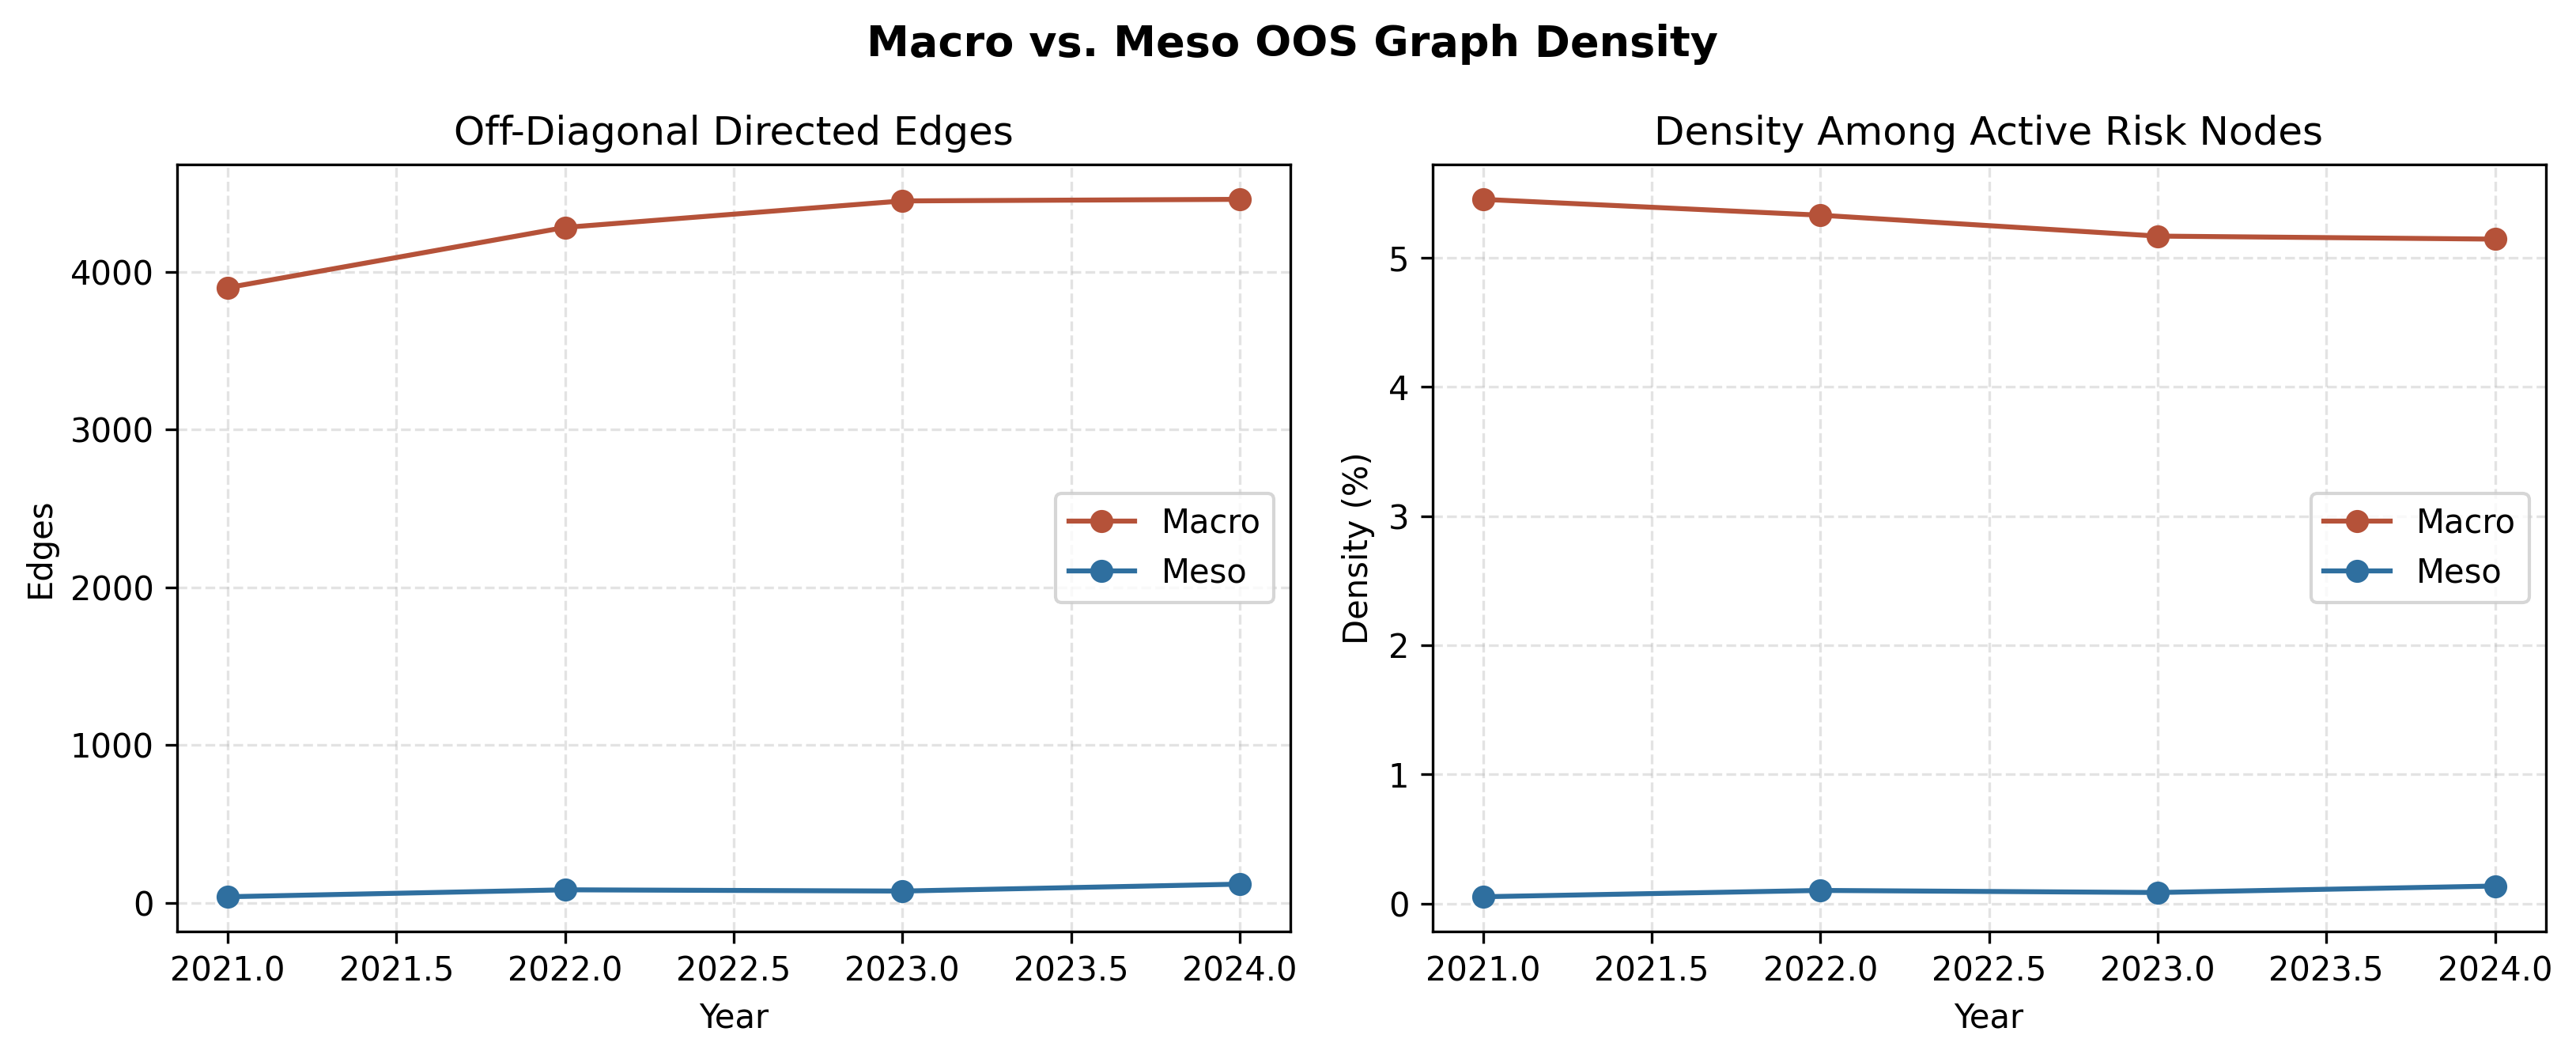
\includegraphics[width=0.92\textwidth]{graph_density_macro_meso.png}
    \caption[Macro versus Meso graph density]{Empirical graph-density comparison for the OOS years, generated from the Macro and Meso graph-diagnostics CSV files.}
    \label{fig:graph_density_macro_meso}
\end{figure}

% ==========================================
% ==========================================
\section{DYNAMIC PORTFOLIO BACKTESTING EXTENSION}
% ==========================================
The forecasting results establish that the Meso topology-only ST-GAT improves cross-sectional return and volatility prediction relative to the identity baseline. However, a statistically better forecast does not automatically imply a tradable investment strategy. To evaluate whether the model produces economically meaningful signals, we extend the forecasting output into a monthly rebalanced portfolio backtest. This section formalizes the signal timing, portfolio construction rules, transaction-cost assumptions, score ablations, benchmark comparison, and top-minus-bottom spread diagnostic.

% --- PORTFOLIO SIGNAL-TIMING TIMELINE ---
\begin{figure}[H]
\centering
\resizebox{0.88\textwidth}{!}{
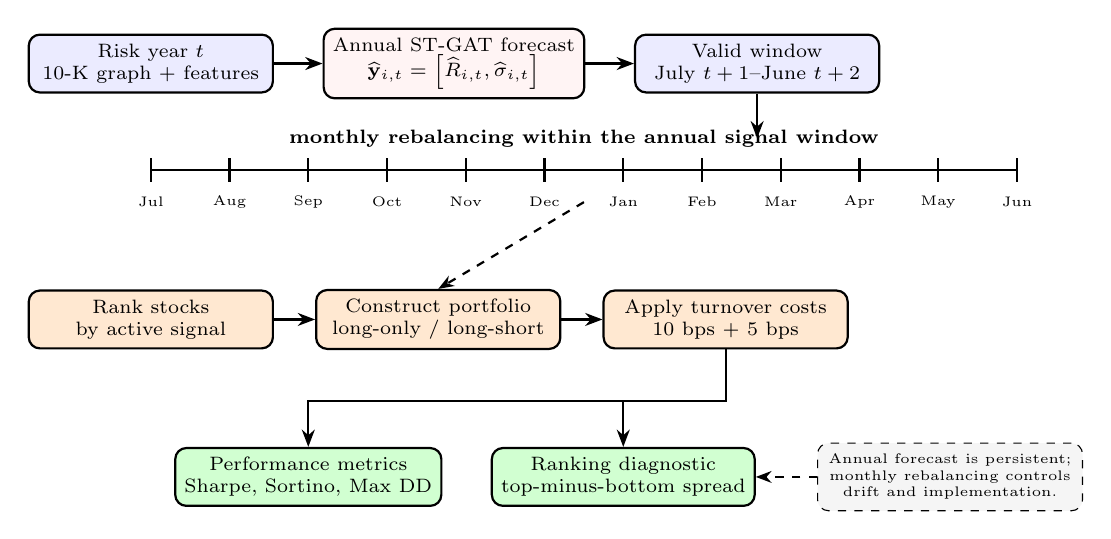
\begin{tikzpicture}[
    topbox/.style={rectangle, rounded corners, draw=black, thick, align=center, minimum width=3.10cm, minimum height=0.72cm, font=\scriptsize, fill=blue!8},
    actionbox/.style={rectangle, rounded corners, draw=black, thick, align=center, minimum width=3.10cm, minimum height=0.72cm, font=\scriptsize, fill=orange!18},
    resultbox/.style={rectangle, rounded corners, draw=black, thick, align=center, minimum width=3.25cm, minimum height=0.72cm, font=\scriptsize, fill=green!18},
    note/.style={rectangle, draw=black, dashed, rounded corners, align=center, font=\tiny, inner sep=4pt, fill=gray!8},
    arrow/.style={thick, -{Stealth[length=2.2mm]}},
    dashedarrow/.style={thick, dashed, -{Stealth[length=2.0mm]}}
]
    % Top row: annual signal timing
    \node[topbox] (observe) at (0,0) {Risk year $t$\\10-K graph + features};
    \node[topbox, fill=pink!18] (forecast) at (3.85,0) {Annual ST-GAT forecast\\$\widehat{\mathbf{y}}_{i,t}=\left[\widehat{R}_{i,t},\widehat{\sigma}_{i,t}\right]$};
    \node[topbox] (window) at (7.70,0) {Valid window\\July $t+1$--June $t+2$};
    \draw[arrow] (observe) -- (forecast);
    \draw[arrow] (forecast) -- (window);

    % Middle row: full July-to-June monthly timeline
    \draw[thick] (0,-1.35) -- (11.0,-1.35);
    \foreach \x/\lab in {0/Jul,1/Aug,2/Sep,3/Oct,4/Nov,5/Dec,6/Jan,7/Feb,8/Mar,9/Apr,10/May,11/Jun}
    {
        \draw[thick] (\x,-1.50) -- (\x,-1.20);
        \node[font=\tiny] at (\x,-1.76) {\lab};
    }
    \node[font=\scriptsize\bfseries] at (5.5,-0.95) {monthly rebalancing within the annual signal window};
    \draw[arrow] (window.south) -- (7.70,-0.95);

    % Bottom row: implementation and evaluation
    \node[actionbox] (rank) at (0,-3.25) {Rank stocks\\by active signal};
    \node[actionbox] (portfolio) at (3.65,-3.25) {Construct portfolio\\long-only / long-short};
    \node[actionbox] (costs) at (7.30,-3.25) {Apply turnover costs\\10 bps + 5 bps};
    \node[resultbox] (metrics) at (2.0,-5.25) {Performance metrics\\Sharpe, Sortino, Max DD};
    \node[resultbox] (spread) at (6.0,-5.25) {Ranking diagnostic\\top-minus-bottom spread};
    \node[note] (timing) at (10.15,-5.25) {Annual forecast is persistent;\\monthly rebalancing controls\\drift and implementation.};

    \draw[arrow] (rank) -- (portfolio);
    \draw[arrow] (portfolio) -- (costs);
    \draw[arrow] (costs.south) -- ++(0,-0.65) -| (metrics.north);
    \draw[arrow] (costs.south) -- ++(0,-0.65) -| (spread.north);
    \draw[dashedarrow] (5.5,-1.76) -- (portfolio.north);
    \draw[dashedarrow] (timing.west) -- (spread.east);
\end{tikzpicture}
}
\caption[Portfolio signal timing]{Portfolio signal timing. Annual ST-GAT predictions remain active over the July-to-June forecast window, while monthly rebalancing controls weight drift, turnover, and implementation costs.}
\label{fig:portfolio_flowchart}
\end{figure}

\subsection{Objective and Signal Choice}
The portfolio extension is designed to answer whether the ST-GAT prediction panel can separate future winners from losers after accounting for realistic implementation frictions. The primary signal source is the Meso ST-GAT output because it is the strongest forecasting specification in Section 8. The identity-baseline predictions are retained as a portfolio benchmark, allowing the analysis to test whether textual peer topology improves allocation quality, not merely predictive loss.

For each firm-year $(i,t)$, the forecast panel contains two model outputs:
\begin{equation}
\widehat{\mathbf{y}}_{i,t}=\left[\widehat{R}_{i,t},\widehat{\sigma}_{i,t}\right],
\end{equation}
where $\widehat{R}_{i,t}$ is predicted forward cumulative return and $\widehat{\sigma}_{i,t}$ is predicted forward annualized volatility. These predictions are generated for the same July-to-June target window used in the supervised learning problem.

\subsection{Annual Signal Persistence and Monthly Rebalancing}
The ST-GAT model produces annual forecasts rather than monthly forecasts. A prediction associated with risk year $t$ is therefore treated as valid from July $t+1$ through June $t+2$. Within this 12-month forecast window, the signal ranking is held fixed unless a new annual prediction becomes available. Monthly rebalancing is nevertheless economically meaningful because it controls weight drift, updates investable eligibility based on available price data, realizes transaction costs, and maintains the intended long, short, and risk-budget exposures.

The timing convention is designed to avoid look-ahead bias. At month-end $m$, the strategy observes the active annual signal available at that date, forms target weights, incurs turnover-based transaction costs, and earns the return from month $m$ to month $m+1$. Thus, the rebalance decision and realized holding-period return are separated by one monthly interval.

\begin{equation}
\mathbf{w}_{m}^{target}=f\left(\mathcal{S}_{m},\mathcal{U}_{m}\right), \qquad
R_{p,m+1}=\sum_{i\in\mathcal{U}_{m}}w_{i,m}^{target}R_{i,m+1}-\text{Cost}_{m},
\end{equation}
where $\mathcal{S}_{m}$ is the active annual signal set and $\mathcal{U}_{m}$ is the investable universe with valid next-month return observations.

\subsection{Score Definitions and Portfolio Ranking}
Because the ST-GAT produces both return and volatility forecasts, we evaluate three alternative scoring rules. The first uses predicted return directly:
\begin{equation}
\text{Score}^{ret}_{i,t}=\widehat{R}_{i,t}.
\end{equation}
The second converts predictions into a risk-adjusted return score:
\begin{equation}
\text{Score}^{ret/vol}_{i,t}=\frac{\widehat{R}_{i,t}}{\max(\widehat{\sigma}_{i,t},0.10)},
\end{equation}
where the 10\% volatility floor prevents unstable weights caused by very small predicted volatility values. The third score uses standardized return and volatility forecasts:
\begin{equation}
\text{Score}^{comp}_{i,t}=z(\widehat{R}_{i,t})-0.5z(\widehat{\sigma}_{i,t}).
\end{equation}
This composite score rewards high predicted return while penalizing high predicted volatility, without imposing the stronger functional form of a return-to-volatility ratio.

\subsection{Long-Only and Long-Short Portfolio Construction}
For each score definition, two strategies are constructed. The first is a long-only top-quintile portfolio. At each rebalance date, stocks are ranked by the active score, and the top 20\% of eligible firms are selected. Within the selected set, weights are scaled inversely by predicted volatility:
\begin{equation}
\tilde{w}_{i,m}=\frac{1/\max(\widehat{\sigma}_{i,t},0.10)}{\sum_{j\in\mathcal{Q}^{top}_{m}}1/\max(\widehat{\sigma}_{j,t},0.10)}.
\end{equation}
A 5\% single-name cap is applied to reduce concentration risk, after which weights are renormalized to sum to one.

The second strategy is a long-short top-minus-bottom quintile portfolio. The top 20\% of stocks by score are held long and the bottom 20\% are held short. The long leg is allocated 50\% gross exposure and the short leg is allocated -50\% gross exposure:
\begin{equation}
\sum_{i\in\mathcal{Q}^{top}_{m}} w_{i,m}=0.5, \qquad
\sum_{i\in\mathcal{Q}^{bottom}_{m}} w_{i,m}=-0.5.
\end{equation}
This design creates an approximately market-neutral cross-sectional ranking test, while still allowing non-zero beta because no explicit beta-neutral optimization is imposed.

\subsection{Transaction Costs, Slippage, and Turnover}
Implementation frictions are modeled using one-way turnover. Let $\mathbf{w}_{m}^{target}$ denote the target weights at rebalance month $m$ and $\mathbf{w}_{m}^{pre}$ denote the drifted weights immediately before rebalancing. Turnover is:
\begin{equation}
\text{Turnover}_{m}=\sum_{i}\left|w^{target}_{i,m}-w^{pre}_{i,m}\right|.
\end{equation}
The total one-way implementation cost is set to 15 bps, consisting of 10 bps transaction cost and 5 bps bid-ask/slippage allowance:
\begin{equation}
\text{Cost}_{m}=0.0015\times \text{Turnover}_{m}.
\end{equation}
Net portfolio return is therefore:
\begin{equation}
R^{net}_{p,m+1}=R^{gross}_{p,m+1}-\text{Cost}_{m}.
\end{equation}
This treatment penalizes both initial portfolio formation and subsequent monthly rebalancing, making the backtest more conservative than a frictionless ranking exercise.

\subsection{Evaluation Metrics}
Portfolio performance is evaluated using total return, annualized return, annualized volatility, Sharpe ratio, Sortino ratio, maximum drawdown, hit rate, average monthly turnover, alpha and beta against SPY, information ratio, and correlation with the benchmark. The Sharpe ratio is the standard mean-variance reward-to-risk measure, while the Sortino ratio focuses on downside risk \citep{sharpe1966mutual, sortino1994performance}.

\subsection{Portfolio Performance Results}
Table \ref{tab:portfolio_results} reports the headline strategies for the metrics currently exported by the backtesting engine. The strongest long-short strategy ranks stocks by predicted return only, rather than by predicted return divided by predicted volatility. This finding is important: although predicted volatility improves the forecasting task, using volatility directly in the denominator can over-penalize high-return opportunities. The return-only signal is therefore the cleanest ranking signal in the current backtest.

\begin{table}[H]
\centering
\caption{Key portfolio backtest results for Meso ST-GAT signals, generated from \texttt{portfolio\_performance\_summary\_ranked.csv}.}
\label{tab:portfolio_results}
\vspace{0.2cm}
\renewcommand{\arraystretch}{1.18}
\small
\begin{tabularx}{\textwidth}{@{}L{4.1cm}ccccc@{}}
\toprule
\textbf{Strategy} & \textbf{Ann. Ret.} & \textbf{Ann. Vol.} & \textbf{Sharpe} & \textbf{Sortino} & \textbf{Max DD} \\
\midrule
GAT Long-Short Return-Only & 7.93\% & 7.47\% & \textbf{1.06} & \textbf{2.01} & \textbf{-6.90\%} \\
GAT Long-Only Return-Only & \textbf{22.71\%} & 21.76\% & 1.04 & 2.24 & -13.99\% \\
SPY Benchmark & 10.74\% & 16.56\% & 0.65 & 1.19 & -23.93\% \\
\bottomrule
\end{tabularx}
\end{table}

The GAT long-short return-only portfolio achieves 7.93\% annualized return with 7.47\% annualized volatility, producing a Sharpe ratio of 1.06 and Sortino ratio of 2.01. Its maximum drawdown is -6.90\%, lower than SPY's -23.93\% over the same exported backtest window. Its beta against SPY is approximately 0.24, indicating that the strategy is not merely a levered market exposure. The GAT long-only return-only portfolio also performs strongly in this academic backtest, generating 22.71\% annualized return, a Sharpe ratio of 1.04, maximum drawdown of -13.99\%, and annualized alpha of approximately 9.85\% against SPY.

\begin{figure}[H]
    \centering
    \includegraphics[width=0.9\textwidth]{GAT_portfolio_output/portfolio_equity_curves.png}
    \caption[Portfolio equity curves]{Monthly rebalanced ST-GAT and identity-baseline portfolio equity curves.}
    \label{fig:portfolio_equity}
\end{figure}

\subsection{Score Ablation Interpretation}
The score ablation shows that the ST-GAT return-only ranking is more effective than the return-over-volatility ranking. This does not contradict the volatility-forecasting improvement documented in Section 8. Rather, it indicates that the predicted volatility output is useful for understanding and controlling risk, but the most direct source of cross-sectional alpha is the predicted return ranking. The composite score performs between the return-only and return-over-volatility specifications, suggesting that moderate volatility penalization is preferable to mechanically dividing by predicted volatility.

This result also clarifies the difference between forecast evaluation and trading evaluation. RMSE and MAE measure point-forecast accuracy, while a portfolio primarily depends on the ordinal separation of expected winners and losers. Therefore, the portfolio section emphasizes Sharpe ratio, drawdown, beta, turnover, and top-minus-bottom spread in addition to predictive metrics.

\subsection{Top-Bottom Spread Diagnostic}
To directly test whether the predicted rankings separate future winners from losers, we compute the monthly average return of the top quintile minus the bottom quintile. This diagnostic is model-agnostic: it does not depend on inverse-volatility weights, portfolio caps, or transaction-cost assumptions. It simply asks whether stocks ranked highly by the signal outperform stocks ranked poorly by the signal in the next month.

\begin{table}[H]
\centering
\caption{Top-minus-bottom spread diagnostics for return-only signals.}
\label{tab:top_bottom_spread}
\vspace{0.2cm}
\renewcommand{\arraystretch}{1.25}
\begin{tabular}{lcccc}
\toprule
\textbf{Signal} & \textbf{Annualized Spread} & \textbf{$t$-stat} & \textbf{$p$-value} & \textbf{Positive Spread Rate} \\
\midrule
ST-GAT Return-Only & \textbf{17.69\%} & \textbf{2.18} & \textbf{0.034} & \textbf{65.2\%} \\
Identity Return-Only & 6.62\% & 1.34 & 0.189 & -- \\
\bottomrule
\end{tabular}
\end{table}

The ST-GAT return-only signal produces a nominally significant 17.69\% annualized top-minus-bottom spread, with $t=2.18$ and $p=0.034$ before adjustment for multiple score/model comparisons. The spread is positive in 65.2\% of evaluated months. By contrast, the identity baseline return-only signal produces a smaller 6.62\% annualized spread with $t=1.34$ and $p=0.189$, which is not statistically significant at conventional levels.

A robustness addendum generated by \codepath{scripts/evaluate_portfolio_inference.py} recomputes spread inference using HAC/Newey-West standard errors with three lags and Benjamini-Hochberg q-values across the six model/score spread tests. Under this more conservative diagnostic, the ST-GAT return-only spread has HAC $t=2.54$, $p=0.011$, and $q=0.049$. This preserves the interpretation that the Meso textual-risk topology improves economic separability, but the evidence should still be read as academic backtest evidence because the sample is short and the exercise is not a live-trading deployment.

\begin{figure}[H]
    \centering
    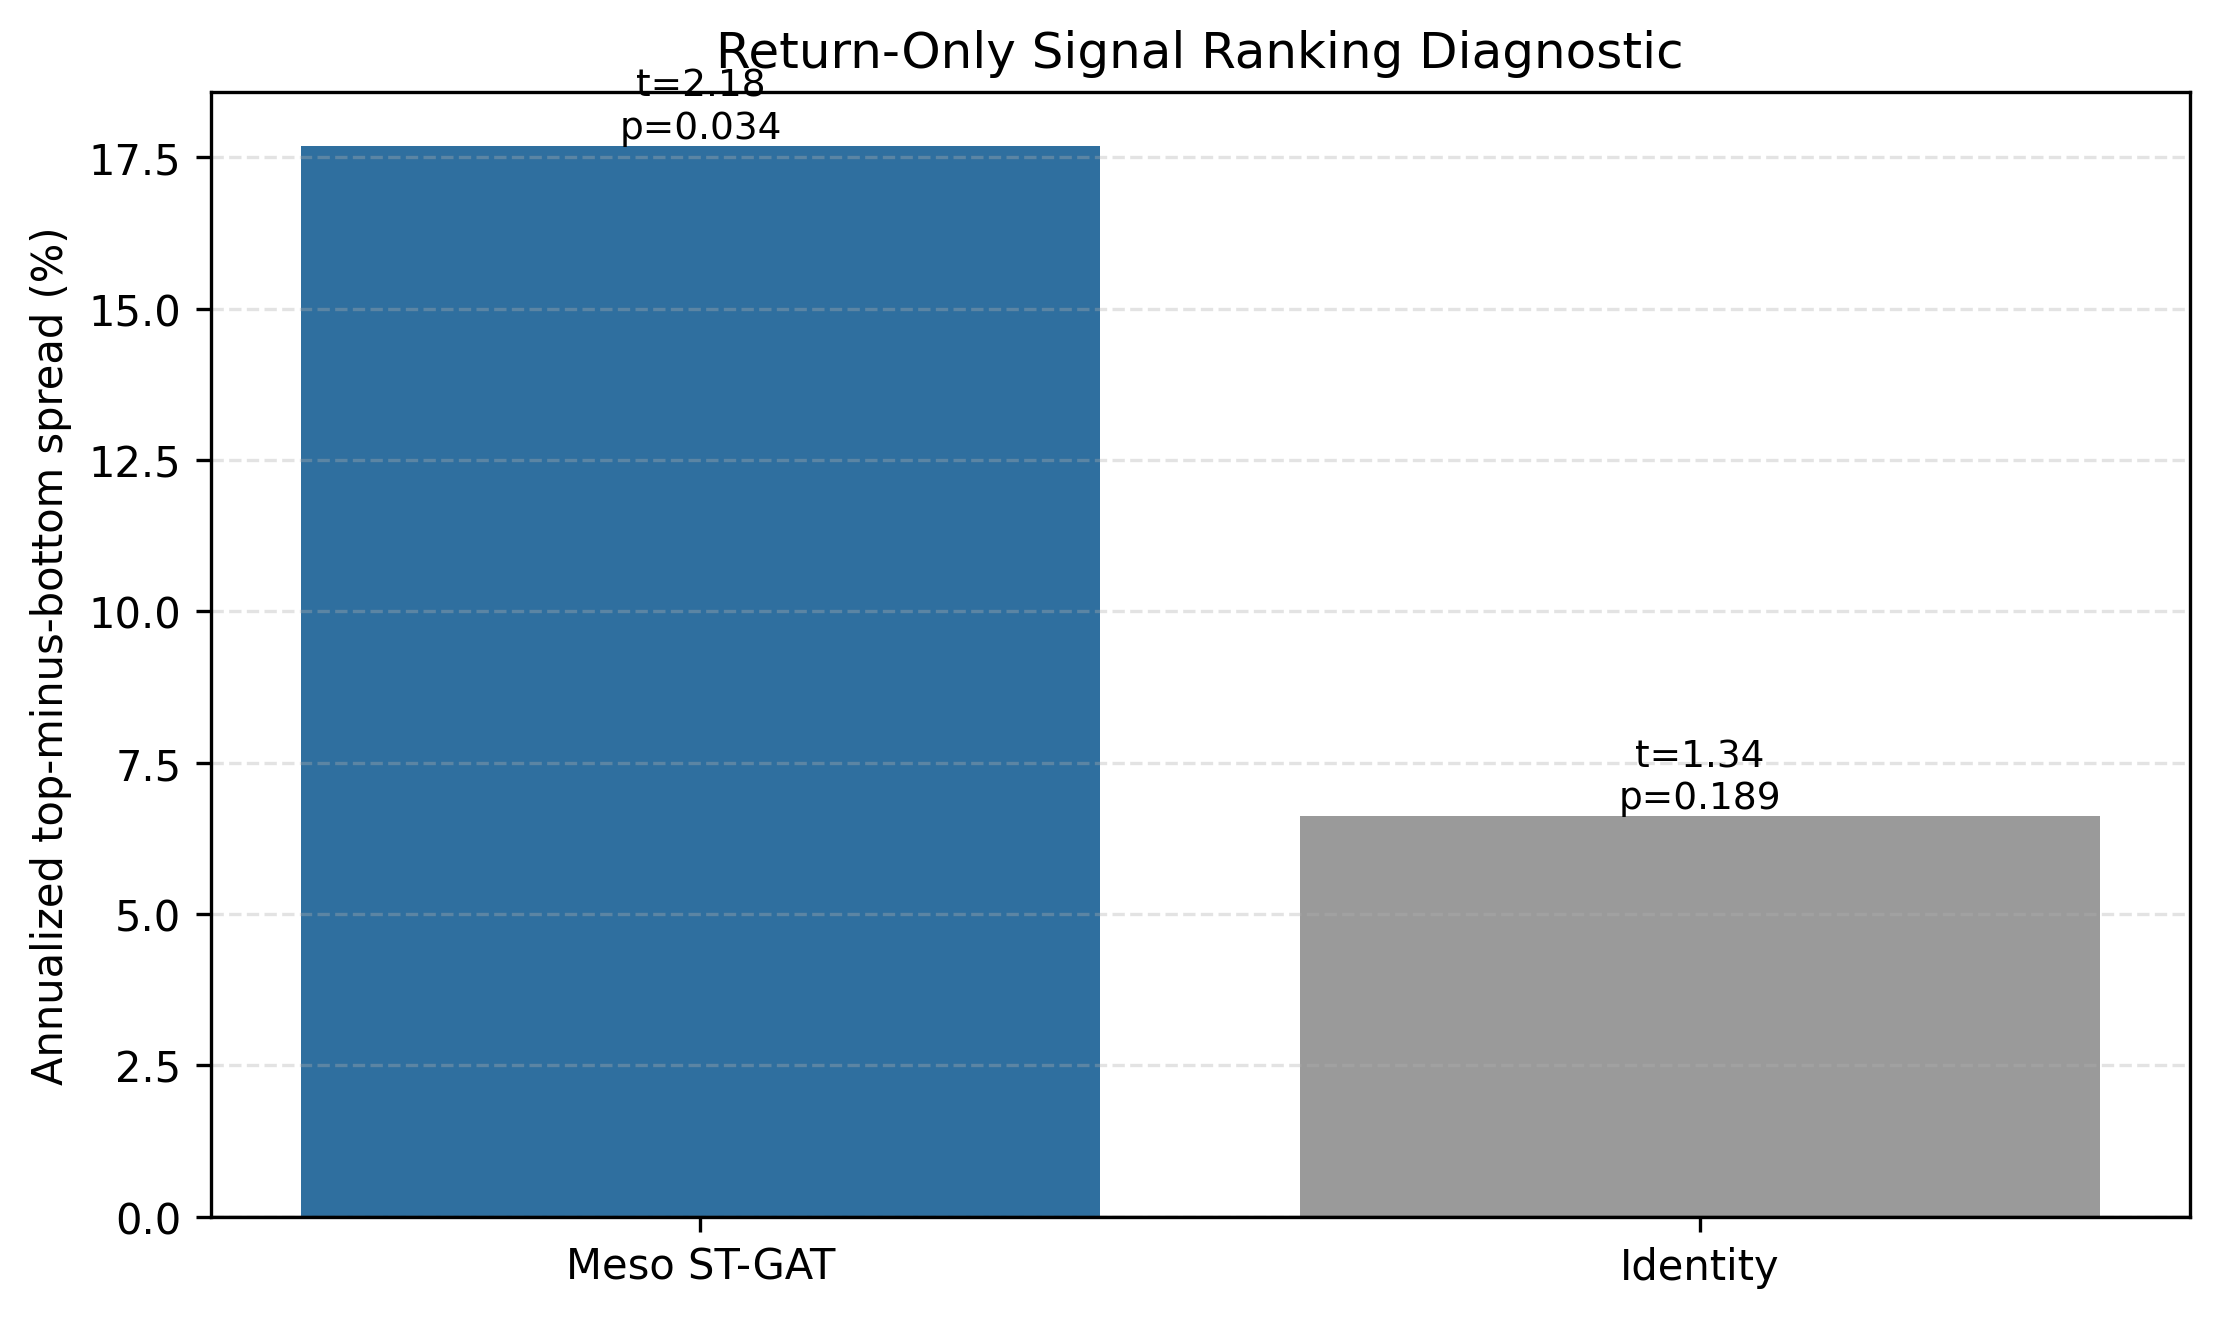
\includegraphics[width=0.72\textwidth]{portfolio_top_bottom_spread.png}
    \caption[Top-minus-bottom spread comparison]{Return-only top-minus-bottom spread diagnostic generated from \texttt{top\_bottom\_spread\_diagnostics.csv}. The reported $p$-values are nominal and not adjusted for multiple score/model comparisons.}
    \label{fig:portfolio_top_bottom_spread}
\end{figure}

\subsection{Portfolio-Level Implications}
The portfolio extension supports three conclusions within an academic backtest setting. First, the Meso ST-GAT signal is economically suggestive: it improves not only statistical forecast metrics but also cross-sectional ranking diagnostics. Second, the best-performing allocation uses predicted return directly, showing that the strongest signal is embedded in the return forecast rather than the return-volatility ratio. Third, monthly rebalancing is compatible with annual predictions when the signal is interpreted as a persistent 12-month forecast and rebalancing is used for risk control and execution rather than signal refresh. These findings motivate further testing of LLM-derived semantic risk topology as an input to systematic equity selection, but they should not be interpreted as live-trading evidence.

% ==========================================
% 9: LIMITATIONS
% ==========================================
\section{LIMITATIONS}

This study identifies several structural and methodological limitations within the proposed Spatio-Temporal Graph Attention Network, the underlying NLP pipeline, and the portfolio extension. First, there is an inherent frequency mismatch between annual 10-K risk disclosures and continuous market dynamics. In the core ST-GAT architecture, this is handled by representing textual risk as an annual cross-sectional graph snapshot. This design is appropriate for one-year-ahead return and volatility forecasting, but it cannot capture intra-year fundamental shocks unless additional higher-frequency textual or event data are incorporated.

Second, the supplemental DAV experiment illustrates the difficulty of mapping annual risk disclosures into daily volatility models. The full BIC horse-race table is currently empty and therefore not treated as verified evidence. The separate DAV peak-event figure set is more informative but still mixed: among 93 figure-derived diagnostics, only 20 show positive peak accuracy improvements and the mean improvement is -2.40\%. This limitation motivates the graph-based cross-sectional architecture and cautions against interpreting annual textual risk scores as high-frequency volatility-trading signals.

Third, the predictive efficacy of the spatial graph topology is bounded by disclosure quality. Firms with boilerplate or near-zero-drift disclosures can introduce persistent but weakly informative links into the adjacency matrix. The strict identity-matrix ablation and the Macro-versus-Meso comparison partially address this issue, but a future implementation should explicitly filter low-drift firms or down-weight stale disclosures when constructing graph topology.

Fourth, the dynamic taxonomy framework relies on a fixed semantic-deviation threshold ($\theta=0.45$). A full longitudinal coverage audit and threshold-sensitivity analysis would be needed to assess stability across the entire 2006--2024 period. There is also residual risk of LLM-induced semantic drift when categories are repeatedly added, merged, or reorganized.

Fifth, secondary validations such as the Spatial Autoregressive network analysis remain constrained by extreme matrix sparsity and small sample sizes. This highlights the difficulty of modeling continuous market dynamics strictly through annualized semantic linkages.

Sixth, the reported portfolio spread $p$-values are nominal. Because multiple score definitions and model variants are evaluated, a stricter confirmatory study should adjust for multiple testing or pre-register a single primary signal before making formal inference.

Seventh, the current validation suite identifies four missing feature values in the enhanced financial matrix. The graph builder handles these through training-year median imputation, which preserves train-only preprocessing, but the missingness should remain documented.

Finally, the portfolio backtest remains an academic backtest rather than a live-trading system. Transaction costs and slippage are included, but borrow constraints, short-sale availability, execution delay, corporate actions, liquidity constraints, and a fully survivorship-bias-free reconstruction of the S\&P 500 universe remain only partially addressed. These limitations should be resolved before interpreting the strategy as deployable capital.
% ==========================================
% 10: CONCLUSION & NEXT STEPS
% ==========================================
\section{CONCLUSION \& NEXT STEPS}

This study develops a comprehensive, LLM-driven framework for transforming lengthy and unstructured SEC Item 1A risk disclosures into quantitative forecasting and portfolio-construction signals. The pipeline extracts risk paragraphs from 10-K filings, maps them into a hierarchical macro--meso taxonomy, converts firm-year disclosures into normalized risk exposure vectors, and uses those vectors to construct dynamic semantic peer graphs.

The central modeling contribution is a topology-only Spatio-Temporal Graph Attention Network with a strict identity-matrix ablation. The full model uses $\mathbf{A}^{full}_{t}=\mathbf{I}+\mathbf{A}^{risk}_{t}$, while the baseline uses $\mathbf{A}^{base}_{t}=\mathbf{I}$. This design isolates the incremental value of textual peer topology beyond each equity's own financial features. In the 2021--2024 OOS period, the Meso ST-GAT outperforms the identity baseline across return and volatility forecasting metrics, improving averaged RMSE from 0.3345 to 0.3001 and averaged Spearman rank from -0.0139 to 0.1701. The strongest improvement occurs in volatility forecasting, where RMSE falls from 0.2240 to 0.1565 and Spearman rank improves from -0.1351 to 0.1770.

Graph diagnostics further clarify why semantic resolution matters. The Macro graph is relatively dense during the OOS period, retaining roughly 3,900--4,460 off-diagonal directed edges per year, while the Meso graph retains only 38--118 edges. The superior performance of the sparse Meso graph supports the interpretation that granular textual-risk categories form high-confidence semantic peer links, whereas broad Macro categories can over-propagate generic disclosure noise.

The portfolio extension demonstrates that the Meso ST-GAT forecasts are statistically useful and economically suggestive in an academic backtest. Annual predictions are held fixed over their July-to-June forecast window and portfolios are rebalanced monthly to control drift, turnover, and implementation costs. The strongest long-short strategy ranks stocks by predicted return, holds the top quintile long and bottom quintile short, and achieves a Sharpe ratio of 1.06, Sortino ratio of 2.01, maximum drawdown of -6.90\%, and beta of 0.24 against SPY. The top-minus-bottom spread diagnostic is nominally significant before multiple-testing adjustment, with a 17.69\% annualized spread, $t=2.18$, and $p=0.034$, compared with an insignificant identity-baseline return-only spread.

Supplemental DAV, Fama-MacBeth, and SAR analyses provide additional economic context but are not treated as verified headline evidence unless their source outputs are regenerated and added to the output manifest. The newly summarized DAV peak diagnostics support only a narrow, event-local interpretation and do not establish broad DAV dominance. The central verified result remains the strict identity-matrix ablation showing that granular Meso textual-risk topology improves the exported ST-GAT forecast panel and portfolio ranking diagnostics relative to own-firm features alone.

Future work should extend the framework in four directions. First, historical constituent reconstruction and delisting-aware price histories should be improved to further mitigate survivorship bias. Second, disclosure staleness and boilerplate intensity should be integrated directly into edge weighting or edge filtering. Third, monthly or quarterly textual/event signals could be added to support genuinely higher-frequency forecasts. Finally, the portfolio engine should be expanded to include borrow constraints, beta-neutral optimization, liquidity-aware execution, and transaction-cost stress testing.
\newpage

% ==========================================
% REFERENCES
% ==========================================
\cleardoublepage
\addcontentsline{toc}{section}{References}
\begin{thebibliography}{99}

    \bibitem[Akiba et~al.(2019)]{akiba2019optuna} Akiba, T., Sano, S., Yanase, T., Ohta, T., \& Koyama, M. (2019). Optuna: A next-generation hyperparameter optimization framework. \textit{Proceedings of the 25th ACM SIGKDD International Conference on Knowledge Discovery \& Data Mining}, 2623--2631.

    \bibitem[Bai et~al.(2018)]{bai2018empirical} Bai, S., Kolter, J. Z., \& Koltun, V. (2018). An empirical evaluation of generic convolutional and recurrent networks for sequence modeling. \textit{arXiv preprint arXiv:1803.01271}.

    \bibitem[Bao and Datta(2014)]{bao2014simultaneously} Bao, Y., \& Datta, A. (2014). Simultaneously discovering and quantifying risk types from textual risk disclosures. \textit{Management Science}, 60(6), 1371--1391.

    \bibitem[Beltagy et~al.(2020)]{beltagy2020longformer} Beltagy, I., Peters, M. E., \& Cohan, A. (2020). Longformer: The long-document transformer. \textit{arXiv preprint arXiv:2004.05150}.

    \bibitem[Blei et~al.(2003)]{blei2003latent} Blei, D. M., Ng, A. Y., \& Jordan, M. I. (2003). Latent Dirichlet allocation. \textit{Journal of Machine Learning Research}, 3, 993--1022.

    \bibitem[Bollerslev(1986)]{bollerslev1986generalized} Bollerslev, T. (1986). Generalized autoregressive conditional heteroskedasticity. \textit{Journal of Econometrics}, 31(3), 307--327.

    \bibitem[Campbell et~al.(2014)]{campbell2014information} Campbell, J. L., Chen, H., Dhaliwal, D. S., Lu, H., \& Steele, L. B. (2014). The information content of mandatory risk factor disclosures in corporate filings. \textit{Review of Accounting Studies}, 19(1), 396--455.

    \bibitem[Campello et~al.(2013)]{campello2013density} Campello, R. J. G. B., Moulavi, D., \& Sander, J. (2013). Density-based clustering based on hierarchical density estimates. \textit{Pacific-Asia Conference on Knowledge Discovery and Data Mining}, 160--172.

    \bibitem[Choi et~al.(2026)]{choi2026llm} Choi, J., Menon, A., \& Taboada, M. (2026). LLM as extractor, embedding as ruler: Alpha generation through semantic changes in corporate disclosures. Working paper.

    \bibitem[Devlin et~al.(2019)]{devlin2019bert} Devlin, J., Chang, M.-W., Lee, K., \& Toutanova, K. (2019). BERT: Pre-training of deep bidirectional transformers for language understanding. \textit{NAACL-HLT}.

    \bibitem[Dyer et~al.(2017)]{dyer2017evolution} Dyer, T., Lang, M., \& Stice-Lawrence, L. (2017). The evolution of 10-K textual disclosure: Evidence from latent Dirichlet allocation. \textit{Journal of Accounting and Economics}, 64(2), 221--245.

    \bibitem[Fama and MacBeth(1973)]{fama1973risk} Fama, E. F., \& MacBeth, J. D. (1973). Risk, return, and equilibrium: Empirical tests. \textit{Journal of Political Economy}, 81(3), 607--636.

    \bibitem[Gao(2016)]{gao2016text} Gao, M. (2016). Text-implied risk factor. Working paper.

    \bibitem[Grundy and Petry(2021)]{grundy2021risk} Grundy, B., \& Petry, S. (2021). 10-K risk-factors quantification and the information content of textual reporting. EFMA 2021.

    \bibitem[Hope et~al.(2016)]{hope2016benefits} Hope, O.-K., Hu, D., \& Lu, H. (2016). The benefits of specific risk-factor disclosures. \textit{Review of Accounting Studies}, 21(4), 1005--1045.

    \bibitem[Huber(1964)]{huber1964robust} Huber, P. J. (1964). Robust estimation of a location parameter. \textit{Annals of Mathematical Statistics}, 35(1), 73--101.

    \bibitem[Jiang et~al.(2026)]{jiang2026finrate} Jiang, Z., et al. (2026). Fin-RATE: A benchmark for LLMs on SEC filings. Working paper.

    \bibitem[Kravet and Muslu(2013)]{kravet2013textual} Kravet, T., \& Muslu, V. (2013). Textual risk disclosures and investors' risk perceptions. \textit{Review of Accounting Studies}, 18(4), 1088--1122.

    \bibitem[Kumar et~al.(2024)]{kumar2024temporal} Kumar, P., Umeorah, N., \& Alochukwu, C. (2024). Temporal graph attention network for volatility forecasting. \textit{Expert Systems with Applications}, 238, 122--135.

    \bibitem[Li(2010)]{li2010textual} Li, F. (2010). Textual analysis of corporate disclosures: A survey of the literature. \textit{Journal of Accounting Literature}, 29, 143--165.

    \bibitem[Liu et~al.(2019)]{liu2019roberta} Liu, Y., Ott, M., Goyal, N., et al. (2019). RoBERTa: A robustly optimized BERT pre-training approach. \textit{arXiv preprint arXiv:1907.11692}.

    \bibitem[Lopez-Lira(2019)]{lopezlira2019risk} Lopez-Lira, A. (2019). Risk factors that matter: Textual analysis of risk disclosures for the cross-section of returns. SSRN 3313663.

    \bibitem[Loughran and McDonald(2011)]{loughran2011liability} Loughran, T., \& McDonald, B. (2011). When is a liability not a liability? Textual analysis, dictionaries, and 10-Ks. \textit{Journal of Finance}, 66(1), 35--65.

    \bibitem[McInnes et~al.(2018)]{mcinnes2018umap} McInnes, L., Healy, J., \& Melville, J. (2018). UMAP: Uniform manifold approximation and projection for dimension reduction. \textit{arXiv preprint arXiv:1802.03426}.

    \bibitem[Naimoli et~al.(2023)]{naimoli2023realized} Naimoli, A., Gerlach, R., \& Storti, G. (2023). Realized EGARCH-X with exogenous variables. \textit{Journal of Financial Econometrics}, 21(2), 345--378.

    \bibitem[Nelson(1991)]{nelson1991conditional} Nelson, D. B. (1991). Conditional heteroskedasticity in asset returns: A new approach. \textit{Econometrica}, 59(2), 347--370.

    \bibitem[Niu et~al.(2024)]{niu2024dynamic} Niu, H., et al. (2024). Dynamic graph construction for financial GNNs: Challenges and opportunities. \textit{IEEE Transactions on Neural Networks and Learning Systems}, 35(4), 512--526.

    \bibitem[Reimers and Gurevych(2019)]{reimers2019sentencebert} Reimers, N., \& Gurevych, I. (2019). Sentence-BERT: Sentence embeddings using Siamese BERT-networks. \textit{EMNLP}.

    \bibitem[Sharpe(1966)]{sharpe1966mutual} Sharpe, W. F. (1966). Mutual fund performance. \textit{Journal of Business}, 39(1), 119--138.

    \bibitem[Sortino and Price(1994)]{sortino1994performance} Sortino, F. A., \& Price, L. N. (1994). Performance measurement in a downside risk framework. \textit{Journal of Investing}, 3(3), 59--64.

    \bibitem[Stevens Institute of Technology(2020)]{stevens2020financial} Stevens Institute of Technology. (2020). Financial disclosure risk factor extension of Fama-French three-factor model. Working paper.

    \bibitem[Veli\v{c}kovi\'{c} et~al.(2018)]{velickovic2018graph} Veli\v{c}kovi\'{c}, P., Cucurull, G., Casanova, A., Romero, A., Li\`{o}, P., \& Bengio, Y. (2018). Graph attention networks. \textit{International Conference on Learning Representations}.

    \end{thebibliography}

\newpage

\appendix
\renewcommand{\thesection}{\Alph{section}}

% ==========================================
\section{Econometric Baseline Specification (DAV Model)}
% ==========================================
To establish a traditional econometric comparison for textual risk integration, the repository includes a Disclosure Augmented Volatility (DAV) model. The DAV framework extends a standard Exponential GARCH (EGARCH) model by introducing textual risk scores as exogenous variables (EGARCH-X). This appendix is supplemental. The aggregate DAV benchmark CSV is empty in the current repository state, so the final report does not make aggregate DAV BIC-improvement claims.

\subsection{Data Sources and Preprocessing}
The model evaluates the 2020--2025 temporal regime. Daily adjusted closing prices were sourced via Yahoo Finance to calculate realized continuous returns ($r_t$). The textual risk signals utilized the granular Meso-level risk matrices derived from the 10-K filings. To align the annual reporting frequency of 10-Ks with daily trading data, the annual risk scores were forward-filled, creating a daily step-function vector for the risk level ($S_t$) and a discrete difference vector for the risk shock ($dS_t$).

\subsection{Mathematical Formulation}
The DAV model is specified as an EGARCH(1,1)-X process. Unlike standard GARCH, the EGARCH framework models the natural logarithm of the conditional variance ($\ln(h_t)$), ensuring positive volatility without enforcing artificial non-negativity constraints on the coefficients. It also captures the asymmetric ``leverage effect'' of negative returns.

The textual risk factors are embedded directly into the conditional variance equation:

\begin{equation}
\ln(h_t) = \omega + \beta \ln(h_{t-1}) + \alpha (|z_{t-1}| - \mathbf{E}[|z|]) + \gamma z_{t-1} + \delta_1 S_t + \delta_2 dS_t
\end{equation}

Where:
\begin{itemize}
    \item $h_t$ is the conditional variance at time $t$.
    \item $z_{t-1}$ is the standardized residual $\frac{\epsilon_{t-1}}{\sqrt{h_{t-1}}}$.
    \item $\gamma$ captures the asymmetric leverage effect of return shocks.
    \item $\delta_1$ measures the persistent ``Level Effect'' of the firm's textual risk score.
    \item $\delta_2$ captures the transient ``Shock Effect'' representing year-over-year changes in disclosure.
\end{itemize}

The models were optimized using the L-BFGS-B algorithm to minimize the negative log-likelihood of the Gaussian distribution. Model selection was governed by the Bayesian Information Criterion (BIC), which severely penalizes models for adding uninformative parameters.

\subsection{Results and Discussion}
The original full-sample DAV horse-race is designed to compare GARCH, EGARCH, and DAV/EGARCH-X by likelihood-based criteria such as BIC. Because \codepath{outputs/econometrics/dav_benchmark_analysis/benchmark_metrics.csv} is empty, the final report omits case-specific BIC-improvement values and treats the full benchmark as a deferred validation task.

The newly added \codepath{outputs/econometrics/dav_peak_analysis/} folder contains a separate peak-event diagnostic rather than the full BIC benchmark table. Each PNG compares a GARCH baseline with a text-augmented DAV curve around the top four distinct volatility events for one ticker--risk pair. Because the peak-analysis folder contains figures but not the original estimation table, the repository now includes \codepath{scripts/summarize_dav_peak_analysis.py}, which parses the existing PNG titles and writes an auditable summary to \codepath{outputs/econometrics/dav_peak_analysis/dav_peak_summary.csv} and \codepath{docs/dav_peak_analysis_summary.md}.

\begin{table}[H]
\centering
\caption{DAV peak-event diagnostic summary derived from 93 figure artifacts.}
\label{tab:dav_peak_summary}
\vspace{0.2cm}
\renewcommand{\arraystretch}{1.18}
\begin{tabular}{lc}
\toprule
\textbf{Diagnostic} & \textbf{Value} \\
\midrule
Peak-event figures scanned & 93 \\
Figure-title improvements parsed & 93 \\
Positive DAV peak improvements & 20 \\
Negative DAV peak improvements & 73 \\
Mean peak accuracy improvement & -2.40\% \\
Median peak accuracy improvement & -1.91\% \\
Standard deviation & 2.95 percentage points \\
Range & -11.74\% to 3.03\% \\
\bottomrule
\end{tabular}
\end{table}

\begin{table}[H]
\centering
\caption{Largest positive DAV peak-event improvements in the available figure set.}
\label{tab:dav_peak_top_positive}
\vspace{0.2cm}
\renewcommand{\arraystretch}{1.12}
\small
\begin{tabularx}{\textwidth}{@{}L{1.5cm}Y Y r@{}}
\toprule
\textbf{Ticker} & \textbf{Macro Risk} & \textbf{Meso Risk} & \textbf{Improvement} \\
\midrule
SHW & Global Economic \& Geopolitical Risk & International Operations and Market-Specific Risks & 3.03\% \\
NOW & Stock Price Volatility & Market and Performance Expectations Volatility & 2.69\% \\
WFC & Cybersecurity \& Data Protection & Cybersecurity Incident \& Breach Risk & 2.36\% \\
KO & Supply Chain \& Operations & Third-Party Dependency and Outsourcing Risks & 1.99\% \\
META & Competitive \& Market Risk & Disruption of Traditional Business Models & 1.61\% \\
\bottomrule
\end{tabularx}
\end{table}

\textbf{Interpretation.} The peak-event evidence weakens, rather than strengthens, any broad claim that annual textual risk scores systematically improve standalone daily volatility models. Only 20 of the 93 figure-derived diagnostics are positive, and the cross-figure mean is negative. The correct academic interpretation is therefore narrow: DAV-style textual volatility augmentation may be useful for selected firm--risk episodes, but the available peak-event artifacts do not support a general statement that DAV dominates a conventional volatility baseline. This reinforces the central design choice of the project: the main verified contribution is the cross-sectional semantic-risk topology and identity-matrix ST-GAT ablation, while DAV remains a supplemental diagnostic for frequency-mismatch and event-local behavior.

\newpage

% ==========================================
\section{Econometric Baseline Specification (Fama-MacBeth Regressions)}
% ==========================================
To evaluate whether the textually derived Meso-level risk vulnerabilities may carry cross-sectional return information, the repository includes a standard Fama-MacBeth (1973) two-stage regression framework. Unlike the DAV model, which analyzes isolated time-series volatility, the Fama-MacBeth methodology cross-sectionally evaluates whether exposure to specific natural-language risk factors is associated with forward returns. The final report treats this as a methodological extension because the source CSV for the numerical Fama-MacBeth table is absent from the output manifest.

\subsection{Data Sources and Mathematical Formulation}
The analysis utilizes the granular Meso-level risk scores extracted from the annual 10-K filings. To align with standard asset pricing literature, these annual risk exposures are held constant over the subsequent 12 months and regressed against one-month forward continuous returns ($r_{i, t+1}$), calculated using adjusted closing prices from Yahoo Finance over the 2020--2025 temporal regime. To overcome the high dimensionality and sparsity of the Meso-risk matrix (where the number of textual parameters $K$ exceeds the cross-sectional equity universe $N$ for specific months), the models are specified as univariate regressions.

\textbf{Stage 1: Cross-Sectional Regressions} \\
For each month $t$, a cross-sectional Ordinary Least Squares (OLS) regression is estimated across all active firms $i$:
\begin{equation}
r_{i, t+1} = \alpha_t + \lambda_{k,t} S_{i,k,t} + \epsilon_{i,t+1} \quad \text{for } i = 1, \dots, N_t
\end{equation}
Where $S_{i,k,t}$ is the textual exposure of firm $i$ to Meso-risk factor $k$ at time $t$, and $\lambda_{k,t}$ is the estimated cross-sectional risk premium.

\textbf{Stage 2: Time-Series Averaging} \\
The final risk premium ($\hat{\lambda}_k$) is computed as the time-series average of the monthly estimates:
\begin{equation}
\hat{\lambda}_k = \frac{1}{T} \sum_{t=1}^T \hat{\lambda}_{k,t}
\end{equation}
Standard errors are corrected using the Newey-West estimator with a 3-month lag structure, producing robust $t$-statistics to control for autocorrelation and heteroskedasticity.

\subsection{Validation Status and Interpretation}
The implemented Fama-MacBeth design is suitable as a future robustness layer for the Meso taxonomy, but the current final report does not report risk-premium coefficients, $t$-statistics, or $p$-values because the corresponding source table is absent. A complete archival version should regenerate the coefficient table from \codepath{src/econometrics/fmb_risk_premium.py}, add the result CSV to \codepath{outputs/econometrics/}, and then update the output manifest. Until that table is available, the Fama-MacBeth module is interpreted as a validation design rather than empirical evidence for priced textual risk factors.

\newpage

% ==========================================
\section{Risk Contagion Network Analysis}
% ==========================================

\subsection{Objective and Motivation}
To validate the practical utility of the evolved taxonomy, we examine whether textual risk disclosure similarities in 10-K filings can predict risk contagion—specifically the synchronization of volatility—within the stock market. We hypothesize that firms sharing similar "risk signatures" in their disclosures (textual peers) will exhibit correlated stock price volatility.

\subsection{Network Construction Methodology}
We transform raw 10-K disclosures into a quantitative risk spillover model through a multi-stage pipeline:

\subsubsection{Risk Exposure Vectors and Similarity}
For each firm $i$ at time $t$, we define a Risk Exposure Vector $\mathbf{R}_{i,t}$:
\begin{equation}
    \mathbf{R}_{i,t} = (w_{i,t,1}, w_{i,t,2}, \dots, w_{i,t,K})
\end{equation}
where $w_{i,t,k}$ represents the normalized count of risk factors assigned to meso-category $k$. The similarity between any two firms $i$ and $j$ is computed using cosine similarity:
\begin{equation}
    \text{sim}(\mathbf{R}_{i}, \mathbf{R}_{j}) = \frac{\mathbf{R}_{i} \cdot \mathbf{R}_{j}}{\|\mathbf{R}_{i}\| \|\mathbf{R}_{j}\|}
\end{equation}

\subsubsection{\texorpdfstring{Spatial Weights Matrix ($\mathbf{W}$)}{Spatial Weights Matrix (W)}}
To define the network topology, we construct a Binary Adjacency matrix $\mathbf{A}_{i,j}$ based on a similarity threshold $\tau$:
\begin{equation}
    \mathbf{A}_{i,j} =
    \begin{cases}
      1 & \text{if } \text{sim}(\mathbf{R}_{i}, \mathbf{R}_{j}) > \tau \\
      0 & \text{otherwise}
    \end{cases}
\end{equation}
A value of 1 indicates a ``Risk Peer'' relationship exists. This is then row-normalized to create the Spatial Weights Matrix $\mathbf{W}_{i,j}$:
\begin{equation}
    \mathbf{W}_{i,j} = \frac{\mathbf{A}_{i,j}}{\sum_{j=1}^n \mathbf{A}_{i,j}}
\end{equation}

\subsection{Spatial Autoregressive (SAR) Framework}
We integrate the NLP-derived risk network with 2023 market price data using a Spatial Autoregressive (SAR) model:
\begin{equation}
    \mathbf{y} = \rho \mathbf{W}\mathbf{y} + \boldsymbol{\alpha} + \boldsymbol{\epsilon}
\end{equation}
Where:
\begin{itemize}
    \item $\mathbf{y}$: The dependent variable, represented by annualized realized volatility in the intended SAR validation design.
    \item $\mathbf{W}$: The \textbf{Spatial Weights Matrix} derived from the evolved taxonomy.
    \item $\rho$ (Rho): The \textbf{Spatial Lag coefficient}, measuring the ``contagion'' effect—how much a firm's volatility is influenced by the volatility of its textual peers.
    \item $\boldsymbol{\alpha}$: The \textbf{baseline idiosyncratic volatility} of a firm, capturing the expected level of risk that remains constant regardless of the spillover effects or contagion within the textual risk network.
\end{itemize}

\subsection{Validation Status and Interpretation}
No source output table for the SAR result is present in the current output manifest, so the final report does not report SAR coefficients, $p$-values, or explanatory power as empirical findings. The SAR framework remains useful as a future network-validation extension: a documented rerun can test whether firms connected by textual-risk similarity also exhibit volatility co-movement after appropriate controls. In the current submission, the SAR appendix is therefore a methodological bridge between semantic peer construction and econometric network validation, not confirmatory evidence.

\newpage

\section{Representative Risk Taxonomy (Sample)}
Due to the high dimensionality and breadth of the evolved risk taxonomy, Table~\ref{tab:risk_taxonomy} presents a representative excerpt of the system's output. This sample illustrates the hierarchical mapping between established \textbf{Macro Categories} and the more granular \textbf{Meso Categories} (Micro-level).
\small
\begin{longtable}{@{}L{0.31\textwidth}L{0.63\textwidth}@{}}
\caption{Extracted Risk Taxonomy: Macro and Micro Categories} \label{tab:risk_taxonomy} \\
\toprule
\textbf{Macro Category} & \textbf{Micro Categories} \\ \midrule
\endfirsthead
\multicolumn{2}{c}%
{{\bfseries \tablename\ \thetable{} -- continued from previous page}} \\
\toprule
\textbf{Macro Category} & \textbf{Micro Categories} \\ \midrule
\endhead
\midrule \multicolumn{2}{r}{{Continued on next page}} \\
\endfoot
\bottomrule
\endlastfoot

Key Person and Succession Risk & Executive Leadership and Critical Function Dependency Risk, Executive Leadership Dependency and Transition Risk \\ \hline
Commodity Price \& Supply Chain Volatility & Raw Material Input Cost Inflation, Human Capital \& Labor Market Disruption \\ \hline
Strategic and Operational Market Vulnerabilities & Intellectual Property and Innovation Competition, Regulatory and Reimbursement Environment \\ \hline
Contractual \& Regulatory Performance Risk & U.S. Government Funding \& Procurement Dependency Risk, Government Contracting \& Performance Risk \\ \hline
Data Privacy \& Cybersecurity Regulatory Compliance Risk & Regulatory Compliance \& Legal Liability Risk for Personal Data, Cross-Jurisdictional Data Privacy Law Compliance Risk \\ \hline
Human Capital Acquisition \& Retention Risk & Key Personnel Dependency \& Talent Competition Risk, Talent Acquisition \& Retention Risk \\ \hline
Human Capital Management \& Organizational Culture & Talent Development \& Learning Systems, Diversity, Equity, Inclusion \& Belonging (DEIB) Strategy \& Goals \\ \hline
Regulatory, Legal, and Tax Compliance Volatility & Tax Law and Liability Volatility, Tax Policy and Obligation Volatility, Tax Provision and Contingency Volatility \\ \hline
Capital Allocation and Shareholder Returns Governance & Structural and Regulatory Constraints on Capital Deployment, Dividend Policy Discretion and Volatility Risk, Stock Price Volatility and Market Perception Risk, Corporate Governance and Controlling Shareholder Risks \\ \hline
Healthcare Policy, Pricing, and Reimbursement Risk & Government Program Contracting \& Compliance Risk, Reimbursement and Pricing Pressure Risk \\ \hline
Legal, Regulatory, and Insurance Risk Exposure & Insurance Adequacy \& Indemnification Risk, Litigation and Legal Contingency Risk \\ \hline
Strategic \& Market Environment Risk & Global Regulatory \& Food Safety Compliance Risk, Competitive \& Market Dynamics Risk \\ \hline
Intellectual Property Rights \& Exclusivity Management & Patent Portfolio Viability \& Litigation Exposure, Third-Party IP Infringement Claims \& Defense Costs, Loss of Exclusivity and Generic/Biosimilar Competition, Third-Party Intellectual Property Dependencies \& Licensing, Intellectual Property Infringement \& Defense \\ \hline
Product Commercialization and Market Dynamics & Manufacturing, Supply Chain, and Operational Capacity, Clinical Development \& Safety Outcomes, Dependency on Strategic Collaborations and Market Exclusivity \\ \hline
Enterprise Risk Governance \& Disclosure Framework & Regulatory \& Disclosure Evolution Risk, Risk Factor Disclosure Framework \\ \hline
International Trade \& Geopolitical Exposure & Cross-Border Regulatory \& Compliance Complexity, Global Supply Chain \& Market Access Disruption \\ \hline
Counterparty and Credit Risk & Investment Portfolio Valuation and Impairment Risk, Credit Rating Downgrade Risk, Debt Refinancing and Liquidity Risk, Regulatory Capital \& Liquidity Compliance Risk, Customer and Counterparty Credit Exposure \\ \hline
Human Capital \& Workforce Management & Labor Cost \& Workforce Stability, Talent Acquisition, Retention \& Succession, Pandemic-Induced Operational \& Economic Disruption, Workforce Health, Safety, \& Operational Continuity \\ \hline
Strategic Transaction \& Integration Execution Risk & Acquisition Integration \& Synergy Realization Risk, Post-Transaction Integration \& Synergy Realization Risk \\ \hline
Climate \& Environmental Disruption Risk & Physical Operational Disruption from Natural Hazards, Transition \& Regulatory Compliance Risk \\ \hline
Third-Party and Supply Chain Dependency & Manufacturing \& Production Disruption, Third-Party Operational and Performance Risk, Supplier Performance and Continuity Risk \\ \hline
Product \& Brand Integrity and Market Acceptance & Product Safety, Quality, and Public Health Perception, Consumer Preference and Health Perception Risk, Bottler Partnership and System Integrity, Competitive Positioning and Market Dynamics \\ \hline
Business Model and Market Evolution Risk & Product Portfolio and Technology Lifecycle Risk, Competitive Pressure and Market Positioning Risk \\
\end{longtable}

\end{document}
